\documentclass{beamer}
\usepackage[english]{layout}
\usepackage[utf8]{inputenc}
\usepackage[english]{babel}
\usepackage[T1]{fontenc}
\usepackage{amsmath, soul, color, multicol, type1cm, verbatim, latexsym, dsfont, float, listings}
\usepackage[official]{eurosym}
\usepackage{algorithmic}
\usepackage{algorithm2e}
\usepackage{float}
\usepackage{beamerthemesplit}
\usepackage{graphicx}
\usepackage[T1]{fontenc}
\usetheme{Frankfurt}
\usecolortheme{lily}
%\usefonttheme{structuresmallcapsserif}
\usefonttheme{professionalfonts}
\setbeamercovered{transparent}

%NeSI Colors <----------------------------------------------------------------------------
\usecolortheme[RGB={47, 68, 71}]{structure} 
\definecolor{nesidark}{HTML}{2F4447}
\definecolor{nesilight}{HTML}{CED9DF}
\definecolor{nesigrey}{gray}{0.7}
\definecolor{nesilightgrey}{gray}{0.98}
\definecolor{nesidarkgrey}{gray}{0.3}
\definecolor{nesiblue}{HTML}{2B9FC2}
\setbeamercolor{block title}{fg=black,bg=nesigrey}
\setbeamercolor{block body}{bg=nesilightgrey,fg=nesidarkgrey}
\setbeamercolor{block body alerted}{bg=white,fg=black}
\setbeamercolor{alerted text}{bg=white,fg=black}

\setbeameroption{show notes}

\setbeamerfont{title}{size=\huge}
\frenchspacing
\hyphenation{NeSI}

\newenvironment{topcolumns}{\begin{columns}[t]}{\end{columns}}
\newcommand\BackgroundPicture[1]{%
\setbeamertemplate{background}{%
\parbox[c][\paperheight]{\paperwidth}{%
\vfill \hfill \includegraphics[height=0.9\paperheight]{#1}
\hfill \vfill
}}}

\setbeamertemplate{blocks}[default]%[shadow=false]
\setbeamertemplate{footline}[frame number]

\useinnertheme{circles}
\setbeamertemplate{title page}[default][center,rounded=false,shadow=false]
%\setbeamertemplate{title page}[default][center, wd=60mm, colsep=-4bp,rounded=true]

% Fancy Footer Content    <---------------------------------------------------------------
%\setbeamertemplate{footline}{
%   \unilogo
%   \dsglogo
%   \begin{beamercolorbox}[ht=4ex,leftskip=1.4cm,rightskip=.3cm]{author in head/foot}
%    \usebeamercolor{nesiblue}
%    \hrule
%    \vspace{0.1cm}
%    \insertdate \hfill \inserttitle \newline
%    \insertshortauthor \ - \insertshortinstitute \hfill \insertframenumber
%   \end{beamercolorbox}
%   \vspace*{0.1cm}
%} 
% Reference http://joerglenhard.wordpress.com/2011/08/04/beamer-customization-ii-footline-with-multiple-lines/
% http://joerglenhard.wordpress.com/tag/beamer/
% https://github.com/lenhard/ub-beamer

%%%%%%%%%%%%%%%%%%%%%%%%%%%%%%%%%%%%%%%%%%%%%%%%%%%%%%%%%%%%%%%%%%%%%%%%%%%%%%%%%%%%%%%%%%
%%%%%%%%%%%%%%%%%%%%%%%%%%%%%%%%%%%%%%%%%%%%%%%%%%%%%%%%%%%%%%%%%%%%%%%%%%%%%%%%%%%%%%%%%
\title{Introduction to Parallel Computing}
%\subtitle{According to NeSI}
\author{NeSI Computational Science Team \\support@nesi.org.nz}
\date{}

%%%%%%%%%%%%%%%%%%%%%%%%%%%%%%%%%%%%%%%%%%%%%%%%%%%%%%%%%%%%%%%%%%%%%%%%%%%%%%%%%%%%%%%%%%
%%%%%%%%%%%%%%%%%%%%%%%%%%%%%%%%%%%%%%%%%%%%%%%%%%%%%%%%%%%%%%%%%%%%%%%%%%%%%%%%%%%%%%%%%
\begin{document}

{
\setbeamertemplate{background canvas}{
\includegraphics[height=0.99\paperheight]{NeSI_img/Slide00.png}} 
\begin{frame}[plain]
\vspace{1cm}
\titlepage
\end{frame}
}


%\BackgroundPicture{NeSI_img/SlideXX.png}
\begin{frame}
\frametitle{Outline}
\begin{multicols}{2}
   \tableofcontents
 \end{multicols}
 \end{frame}

%%%%%%%%%%%%%%%%%%%%%%%%%%%%%%%%%%%%%%%%%%%%%%%%%%%%%%%%%%%%%%%%%%%%%%%%%%%%%%%%%%%%%%%%%
%%%%%%%%%%%%%%%%%%%%%%%%%%%%%%%%%%%%%%%%%%%%%%%%%%%%%%%%%%%%%%%%%%%%%%%%%%%%%%%%%%%%%%%%%
\section{Story of computing}
%%%%%%%%%%%%%%%%%%%%%%%%%%%%%%%%%%%%%%%%%%%%%%%%%%%%%%%%%%%%%%%%%%%%%%%%%%%%%%%%%%%%%%%%%
%%%%%%%%%%%%%%%%%%%%%%%%%%%%%%%%%%%%%%%%%%%%%%%%%%%%%%%%%%%%%%%%%%%%%%%%%%%%%%%%%%%%%%%%%
%%%%%%%%%%%%%%%%%%%%%%%%%%%%%%%%%%%%%%%%%%%%%%%%%%%%%%%%%%%%%%%%%%%%%%%%%%%%%%%%%%%%%%%%%
\subsection{The beginning}
%%%%%%%%%%%%%%%%%%%%%%%%%%%%%%%%%%%%%%%%%%%%%%%%%%%%%%%%%%%%%%%%%%%%%%%%%%%%%%%%%%%%%%%%%

%%%%%%%%%%%%%%%%%%%%%%%%%%%%%%%%%%%%%%%%%%%%%%%%%%%%%%%%%%%%%%%%%%%%%%%%%%%%%%%%%%%%%%%%%
\frame[t]
{
	\frametitle{Story of computing}
	\framesubtitle{The Beginning}
   \begin{block}{Alan Turing}
   \begin{center}
 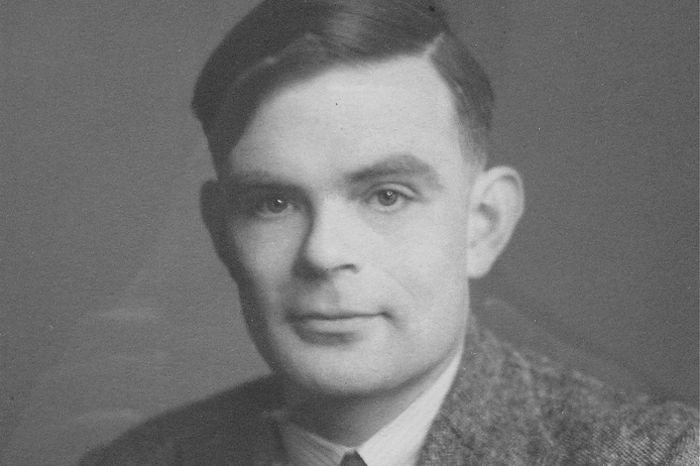
\includegraphics[width=250pt]{fig/turing.jpg}
   \end{center}
  \end{block}

}
%%%%%%%%%%%%%%%%%%%%%%%%%%%%%%%%%%%%%%%%%%%%%%%%%%%%%%%%%%%%%%%%%%%%%%%%%%%%%%%%%%%%%%%%%

%%%%%%%%%%%%%%%%%%%%%%%%%%%%%%%%%%%%%%%%%%%%%%%%%%%%%%%%%%%%%%%%%%%%%%%%%%%%%%%%%%%%%%%%%
\frame[t]
{
	\frametitle{Story of computing}
	\begin{block}{Turing Machine}
   	\begin{itemize}
		\item 	During World War II, Alan Turing, a British mathematician, started to work
		with Britain's code-breaking centre and deciphered Germany's U-boat Enigma, winning 
		the battle of Atlantic! 
	  	\item	He conceived the principles of modern computers and introduced
	  	his famous ``Turing Machine'' in 1936. 
	  	\item ``Turing Machine'' is a hypothetical device
	  	   	\begin{itemize}
	  	   	 	\item It manipulates symbols on a strip of tape based on a table of rules.
	  			\item It could simulate the logic of almost any computer algorithm.
	  		\end{itemize}
   	\end{itemize}	

   	  
	\end{block}
}
%%%%%%%%%%%%%%%%%%%%%%%%%%%%%%%%%%%%%%%%%%%%%%%%%%%%%%%%%%%%%%%%%%%%%%%%%%%%%%%%%%%%%%%%%

%%%%%%%%%%%%%%%%%%%%%%%%%%%%%%%%%%%%%%%%%%%%%%%%%%%%%%%%%%%%%%%%%%%%%%%%%%%%%%%%%%%%%%%%%
\frame[t]
{
	\frametitle{Story of computing}
	\begin{block}{Z1}
   		\begin{itemize}
			\item On the other side of the spectrum Konrad Zuse, 
			a German civil engineer in Berlin, started dreaming of a machine that could do 
			mechanical calculations.
			\item He started working in his parents' apartment and built his 
			first electro-mechanical computer, the Z1, in the same year 1936.
			\item It was a floating point binary mechanical calculator with limited 
			programmability, reading instructions from a perforated 35 mm film.
		\end{itemize}
		
	\end{block}
}
%%%%%%%%%%%%%%%%%%%%%%%%%%%%%%%%%%%%%%%%%%%%%%%%%%%%%%%%%%%%%%%%%%%%%%%%%%%%%%%%%%%%%%%%%

%%%%%%%%%%%%%%%%%%%%%%%%%%%%%%%%%%%%%%%%%%%%%%%%%%%%%%%%%%%%%%%%%%%%%%%%%%%%%%%%%%%%%%%%%
\frame[t]
{
	\frametitle{Story of computing}
   	\begin{block}{Konrad Zuse}
   		\begin{center}
 			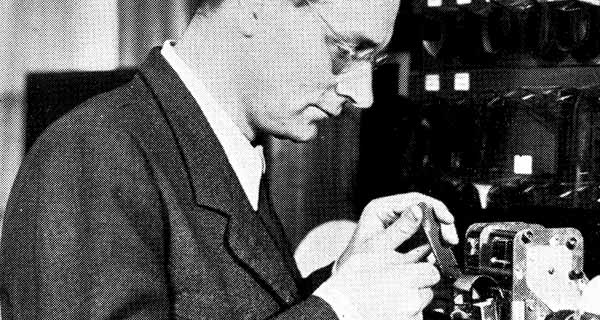
\includegraphics[width=250pt]{fig/zuse.jpg}
   		\end{center}
   		So we have a situation of two people coming from two different 
		backgrounds and laying foundations of computer science. 
  	\end{block}
}
%%%%%%%%%%%%%%%%%%%%%%%%%%%%%%%%%%%%%%%%%%%%%%%%%%%%%%%%%%%%%%%%%%%%%%%%%%%%%%%%%%%%%%%%%


%%%%%%%%%%%%%%%%%%%%%%%%%%%%%%%%%%%%%%%%%%%%%%%%%%%%%%%%%%%%%%%%%%%%%%%%%%%%%%%%%%%%%%%%%
\subsection{Need for speed}
%%%%%%%%%%%%%%%%%%%%%%%%%%%%%%%%%%%%%%%%%%%%%%%%%%%%%%%%%%%%%%%%%%%%%%%%%%%%%%%%%%%%%%%%%

%%%%%%%%%%%%%%%%%%%%%%%%%%%%%%%%%%%%%%%%%%%%%%%%%%%%%%%%%%%%%%%%%%%%%%%%%%%%%%%%%%%%%%%%%
\frame[t]
{
  \frametitle{Story of computing}
    \framesubtitle{Need for speed}
      \begin{block}{Seymour Cray}
   \begin{itemize}
	\item There was great appetite for speed, which was fuelled by the aspirations 
	of an American named Seymour Cray. 
	\item He designed the first supercomputer, the Cray-1, in 1976. He is called the 
	``father of supercomputing''. 
   \end{itemize}
  \end{block}
  
    \begin{center}
  		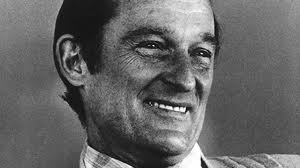
\includegraphics[width=140pt]{fig/cray.jpg}
 	\end{center}
}
%%%%%%%%%%%%%%%%%%%%%%%%%%%%%%%%%%%%%%%%%%%%%%%%%%%%%%%%%%%%%%%%%%%%%%%%%%%%%%%%%%%%%%%%%

%%%%%%%%%%%%%%%%%%%%%%%%%%%%%%%%%%%%%%%%%%%%%%%%%%%%%%%%%%%%%%%%%%%%%%%%%%%%%%%%%%%%%%%%%
\frame[t]
{
  \frametitle{Story of computing}
      \begin{block}{Cray-1} 
        First supercomputers were monolithic in structure and architecture. 
   		\begin{center}
 			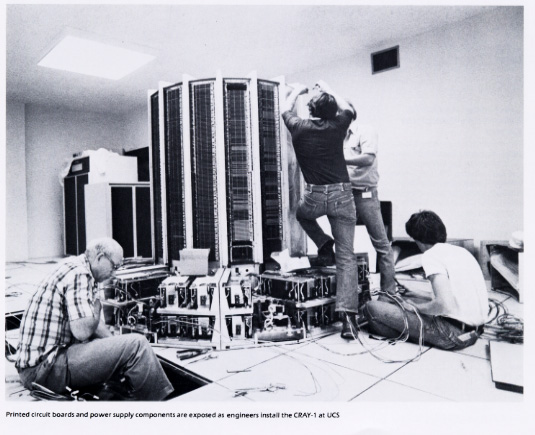
\includegraphics[width=190pt]{fig/cray1-install.jpg}
   		\end{center}  
		
  	\end{block}
  	
  	\note {Cray-2 had only 1 gigaflops peak performance with a cost as high as \$32,000 per
  	megaflops, whereas your PC will have around 40 gigaflops peak performance at \$0.04
  	cost per megaflop (``Flops'' stands for floating point operations per second).} 
}
%%%%%%%%%%%%%%%%%%%%%%%%%%%%%%%%%%%%%%%%%%%%%%%%%%%%%%%%%%%%%%%%%%%%%%%%%%%%%%%%%%%%%%%%%


%%%%%%%%%%%%%%%%%%%%%%%%%%%%%%%%%%%%%%%%%%%%%%%%%%%%%%%%%%%%%%%%%%%%%%%%%%%%%%%%%%%%%%%%%%
%%%%%%%%%%%%%%%%%%%%%%%%%%%%%%%%%%%%%%%%%%%%%%%%%%%%%%%%%%%%%%%%%%%%%%%%%%%%%%%%%%%%%%%%%%
\section{Hegelian dialectics}
%%%%%%%%%%%%%%%%%%%%%%%%%%%%%%%%%%%%%%%%%%%%%%%%%%%%%%%%%%%%%%%%%%%%%%%%%%%%%%%%%%%%%%%%%%
%%%%%%%%%%%%%%%%%%%%%%%%%%%%%%%%%%%%%%%%%%%%%%%%%%%%%%%%%%%%%%%%%%%%%%%%%%%%%%%%%%%%%%%%%%

%%%%%%%%%%%%%%%%%%%%%%%%%%%%%%%%%%%%%%%%%%%%%%%%%%%%%%%%%%%%%%%%%%%%%%%%%%%%%%%%%%%%%%%%%%
%%%%%%%%%%%%%%%%%%%%%%%%%%%%%%%%%%%%%%%%%%%%%%%%%%%%%%%%%%%%%%%%%%%%%%%%%%%%%%%%%%%%%%%%%%
\subsection{Thesis}
%%%%%%%%%%%%%%%%%%%%%%%%%%%%%%%%%%%%%%%%%%%%%%%%%%%%%%%%%%%%%%%%%%%%%%%%%%%%%%%%%%%%%%%%%%
%%%%%%%%%%%%%%%%%%%%%%%%%%%%%%%%%%%%%%%%%%%%%%%%%%%%%%%%%%%%%%%%%%%%%%%%%%%%%%%%%%%%%%%%%%

%%%%%%%%%%%%%%%%%%%%%%%%%%%%%%%%%%%%%%%%%%%%%%%%%%%%%%%%%%%%%%%%%%%%%%%%%%%%%%%%%%%%%%%%%%
\frame[t]
{
  \frametitle{Hegelian dialectics}
    \framesubtitle{Thesis: one}
      \begin{block}{Two rules}
      
      \begin{itemize}
		\item If we look carefully at the history of computing, we could see the Hegelian 
		cycles of thesis and anti-thesis resulting in a synthesis. 
		\item Computing, or even supercomputing 
		started with monolithic machines getting bigger and faster. That was the thesis. 
		\item Two rules emerged to support this model:
		      \begin{itemize}
		      \item Moore's Law
		      \item Amdahl's Law
		      \end{itemize}		
		\end{itemize}
   
  \end{block}
}
%%%%%%%%%%%%%%%%%%%%%%%%%%%%%%%%%%%%%%%%%%%%%%%%%%%%%%%%%%%%%%%%%%%%%%%%%%%%%%%%%%%%%%%%%%

%%%%%%%%%%%%%%%%%%%%%%%%%%%%%%%%%%%%%%%%%%%%%%%%%%%%%%%%%%%%%%%%%%%%%%%%%%%%%%%%%%%%%%%%%%
%%%%%%%%%%%%%%%%%%%%%%%%%%%%%%%%%%%%%%%%%%%%%%%%%%%%%%%%%%%%%%%%%%%%%%%%%%%%%%%%%%%%%%%%%%
\subsubsection{Moore's law}
%%%%%%%%%%%%%%%%%%%%%%%%%%%%%%%%%%%%%%%%%%%%%%%%%%%%%%%%%%%%%%%%%%%%%%%%%%%%%%%%%%%%%%%%%%
%%%%%%%%%%%%%%%%%%%%%%%%%%%%%%%%%%%%%%%%%%%%%%%%%%%%%%%%%%%%%%%%%%%%%%%%%%%%%%%%%%%%%%%%%%

%%%%%%%%%%%%%%%%%%%%%%%%%%%%%%%%%%%%%%%%%%%%%%%%%%%%%%%%%%%%%%%%%%%%%%%%%%%%%%%%%%%%%%%%%%
\frame[t]
{
  \frametitle{Hegelian dialectics}
      \begin{block}{Moore's law}
        \begin{itemize}
			\item Proposed by Gordon E. Moore (co-founder of Intel) in 1965. 
			\item In simple terms the law states that processing speed of
			 computers will double every two years.  
			\item More specifically it stated that the number of transistors on an 
			affordable CPU would double every two years.
			\item Over roughly 50 years from 1961, the number of transistors 
			doubled approximately every 18 months!
        \end{itemize}		
		
  \end{block}
}
%%%%%%%%%%%%%%%%%%%%%%%%%%%%%%%%%%%%%%%%%%%%%%%%%%%%%%%%%%%%%%%%%%%%%%%%%%%%%%%%%%%%%%%%%%

%%%%%%%%%%%%%%%%%%%%%%%%%%%%%%%%%%%%%%%%%%%%%%%%%%%%%%%%%%%%%%%%%%%%%%%%%%%%%%%%%%%%%%%%%
\frame[t]
{
  \frametitle{Hegelian dialectics}
      \begin{block}{Moore's law in airline industry!}
   		\begin{center}
 			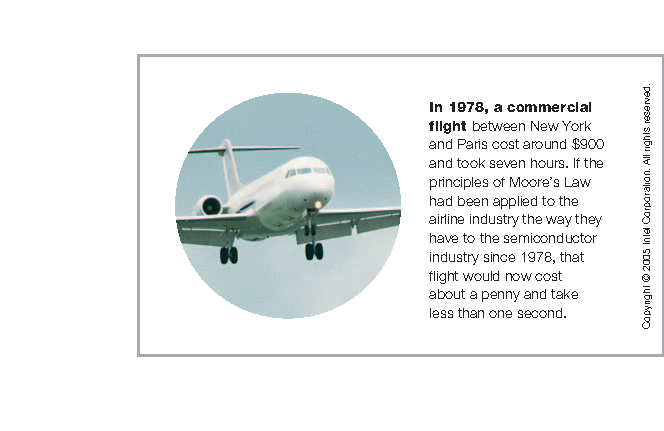
\includegraphics[width=250pt]{fig/ml-flight.pdf}
   		\end{center}  
		
  	\end{block}
}
%%%%%%%%%%%%%%%%%%%%%%%%%%%%%%%%%%%%%%%%%%%%%%%%%%%%%%%%%%%%%%%%%%%%%%%%%%%%%%%%%%%%%%%%%

%%%%%%%%%%%%%%%%%%%%%%%%%%%%%%%%%%%%%%%%%%%%%%%%%%%%%%%%%%%%%%%%%%%%%%%%%%%%%%%%%%%%%%%%%
\frame[t]
{
  \frametitle{Hegelian dialectics}
      \begin{block}{Gordon E. Moore}
   		\begin{center}
 			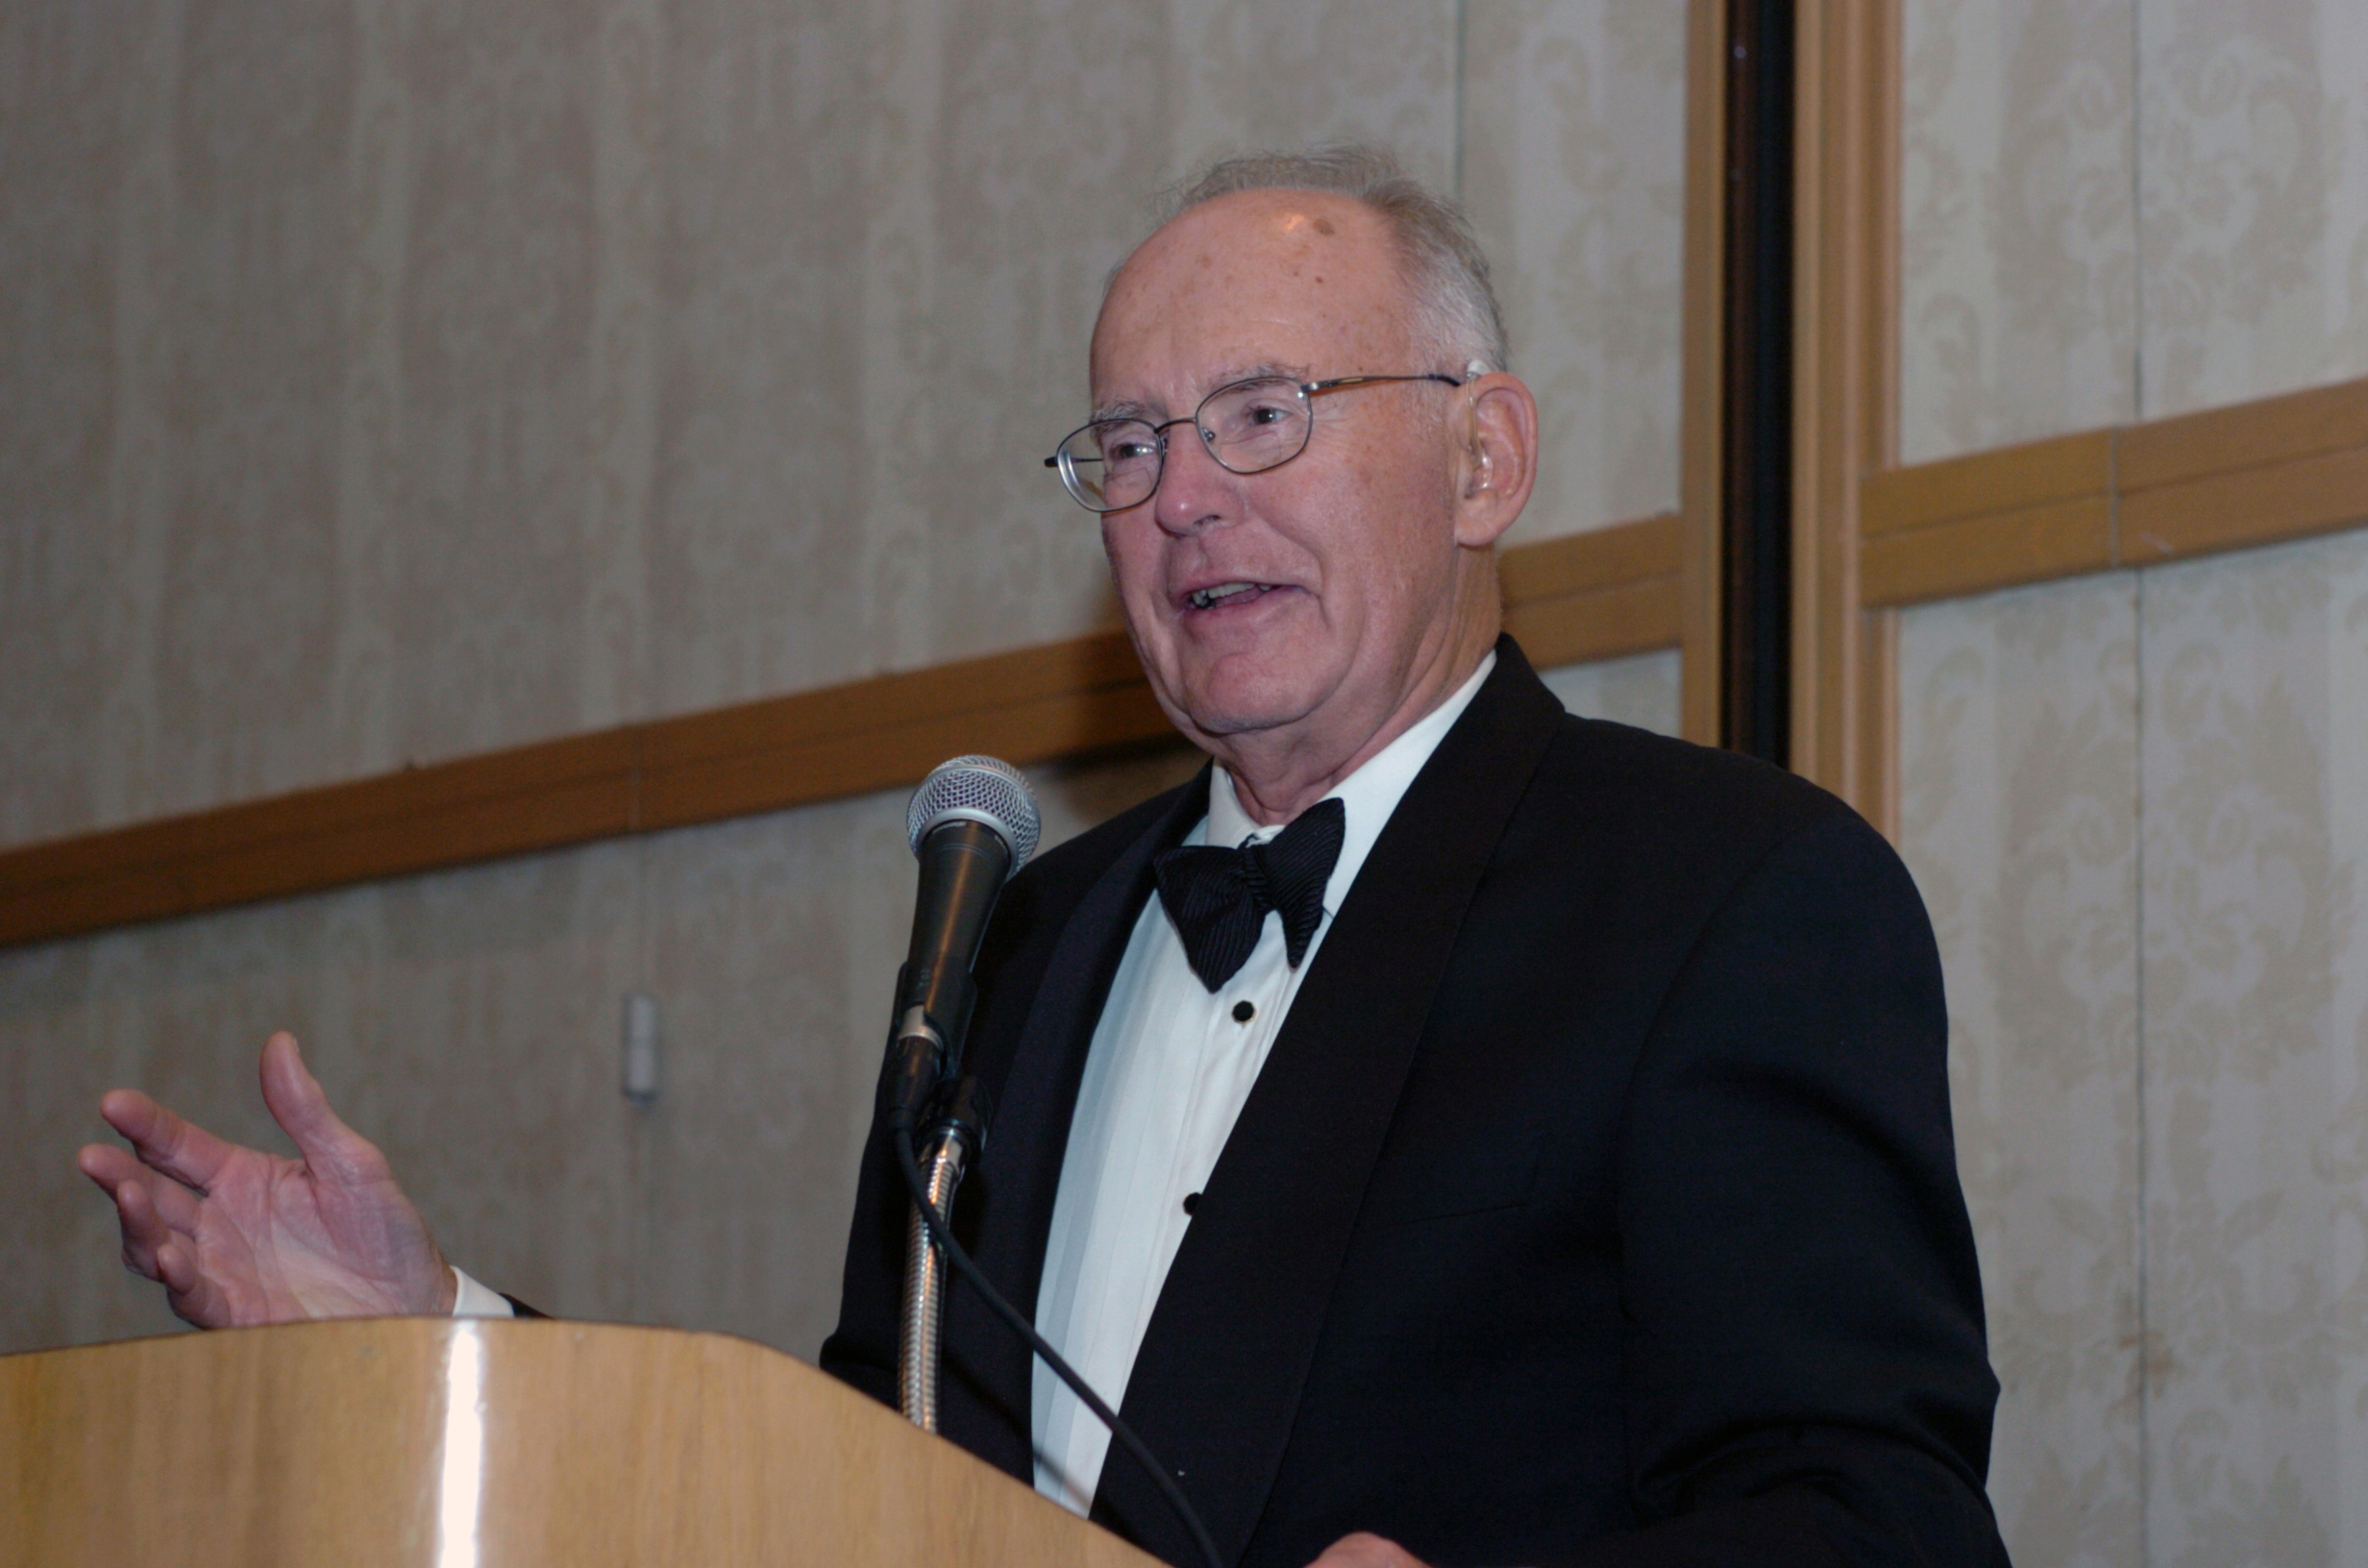
\includegraphics[width=250pt]{fig/moore-2004.jpg}
   		\end{center}  
		
  	\end{block}
}
%%%%%%%%%%%%%%%%%%%%%%%%%%%%%%%%%%%%%%%%%%%%%%%%%%%%%%%%%%%%%%%%%%%%%%%%%%%%%%%%%%%%%%%%%

%%%%%%%%%%%%%%%%%%%%%%%%%%%%%%%%%%%%%%%%%%%%%%%%%%%%%%%%%%%%%%%%%%%%%%%%%%%%%%%%%%%%%%%%%%
%%%%%%%%%%%%%%%%%%%%%%%%%%%%%%%%%%%%%%%%%%%%%%%%%%%%%%%%%%%%%%%%%%%%%%%%%%%%%%%%%%%%%%%%%%
\subsubsection{Amdahl’s law}
%%%%%%%%%%%%%%%%%%%%%%%%%%%%%%%%%%%%%%%%%%%%%%%%%%%%%%%%%%%%%%%%%%%%%%%%%%%%%%%%%%%%%%%%%%
%%%%%%%%%%%%%%%%%%%%%%%%%%%%%%%%%%%%%%%%%%%%%%%%%%%%%%%%%%%%%%%%%%%%%%%%%%%%%%%%%%%%%%%%%%

%%%%%%%%%%%%%%%%%%%%%%%%%%%%%%%%%%%%%%%%%%%%%%%%%%%%%%%%%%%%%%%%%%%%%%%%%%%%%%%%%%%%%%%%%%
\frame[t]
{
  \frametitle{Hegelian dialectics}
      \begin{block}{Amdahl's law}
        \begin{itemize}
			\item Proposed by Gene Amdahl in his 1967 technical paper titled
			``Validity of the single processor approach to achieving large scale 
			computing capabilities''. 
        	\item ``The speedup of a program using multiple processors in parallel 
			computing is limited by the time needed for the sequential fraction of 
			the program.''

			\item The famous Amdahl's equation below is not in this paper, but only a small
			literal description in the 4th paragraph of the 4 page paper!
        \end{itemize}		
		
  \end{block}      
}
%%%%%%%%%%%%%%%%%%%%%%%%%%%%%%%%%%%%%%%%%%%%%%%%%%%%%%%%%%%%%%%%%%%%%%%%%%%%%%%%%%%%%%%%%%

%%%%%%%%%%%%%%%%%%%%%%%%%%%%%%%%%%%%%%%%%%%%%%%%%%%%%%%%%%%%%%%%%%%%%%%%%%%%%%%%%%%%%%%%%
\frame[t]
{
  \frametitle{Hegelian dialectics}
      \begin{block}{Amdahl's equation}
   		\begin{center}
 			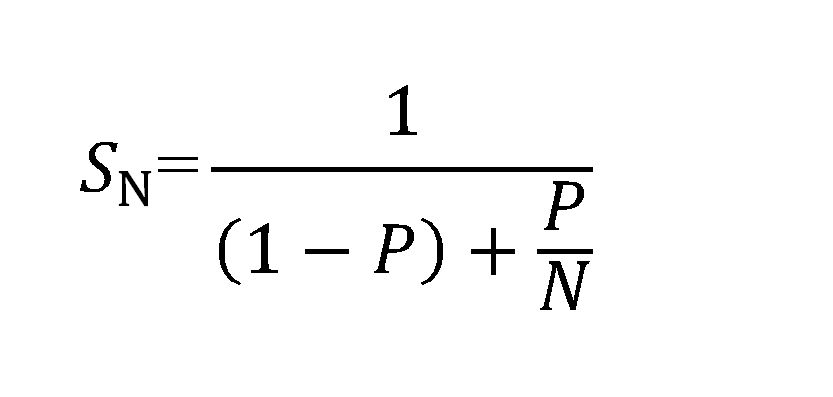
\includegraphics[width=100pt]{fig/amdahl-eq.jpg}
   		 \end{center}
   		 
   		 \begin{itemize}
   		 	\item Where:
   		 	   	\begin{itemize}
   		 		 	\item $P$ is the proportion of a program that can be made parallel.
   		 		 	\item $(1 - P)$ is the proportion that cannot be parallelized.
   		 		 	\item $N$ is the number of processors.
   		 		 	\item $S$ is speedup.
   		 		\end{itemize}
			\item	The idea of Amdahl's law was to show the limitations of 
			parallel computing!
		\end{itemize}
      \end{block}
}
%%%%%%%%%%%%%%%%%%%%%%%%%%%%%%%%%%%%%%%%%%%%%%%%%%%%%%%%%%%%%%%%%%%%%%%%%%%%%%%%%%%%%%%%%

%%%%%%%%%%%%%%%%%%%%%%%%%%%%%%%%%%%%%%%%%%%%%%%%%%%%%%%%%%%%%%%%%%%%%%%%%%%%%%%%%%%%%%%%%
\frame[t]
{
  \frametitle{Hegelian dialectics}
   		\begin{center}
 			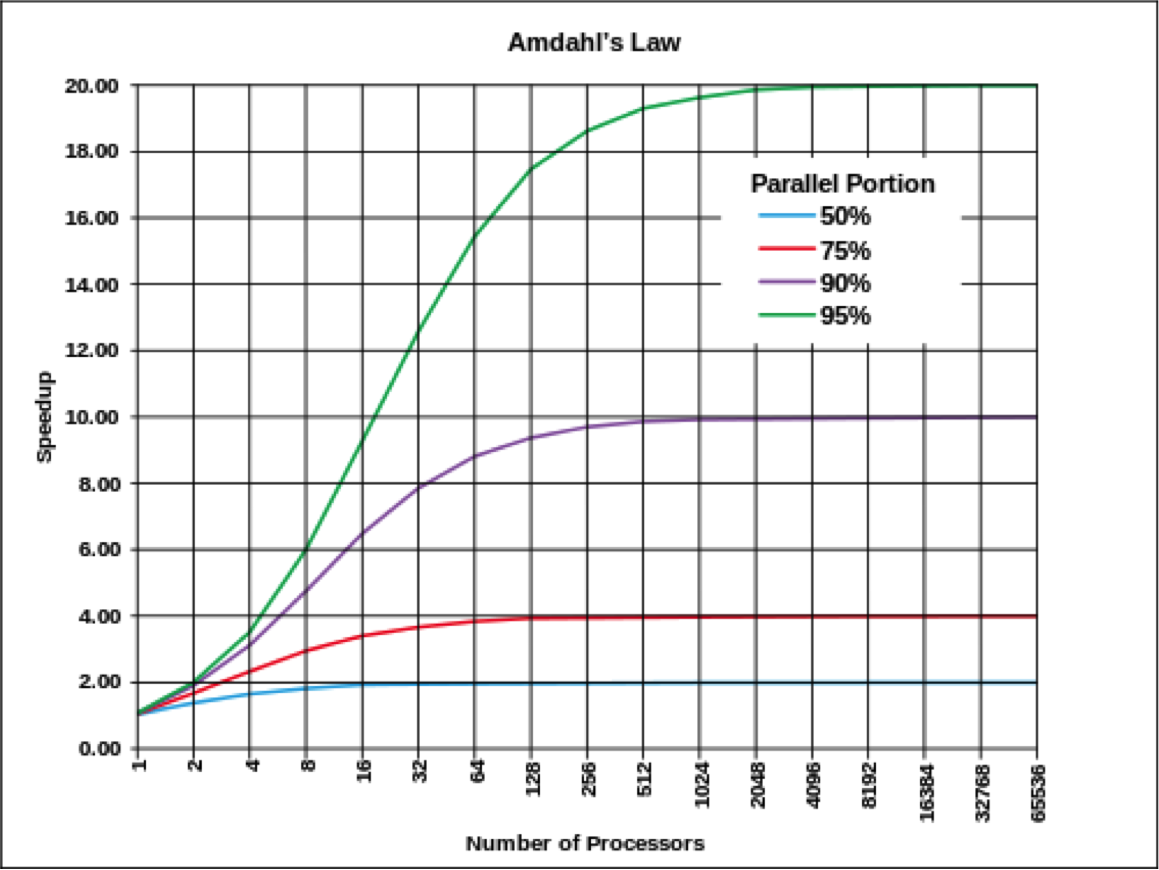
\includegraphics[width=180pt]{fig/amdahl-graph.png}
   		\end{center}  
   		 \begin{itemize}
   		 	\item Not even considering the overheads of parallelisation.
			\item If parallelisation cannot be done evenly, results will be much worse!
   		 \end{itemize}
}
%%%%%%%%%%%%%%%%%%%%%%%%%%%%%%%%%%%%%%%%%%%%%%%%%%%%%%%%%%%%%%%%%%%%%%%%%%%%%%%%%%%%%%%%%


%%%%%%%%%%%%%%%%%%%%%%%%%%%%%%%%%%%%%%%%%%%%%%%%%%%%%%%%%%%%%%%%%%%%%%%%%%%%%%%%%%%%%%%%%%
%%%%%%%%%%%%%%%%%%%%%%%%%%%%%%%%%%%%%%%%%%%%%%%%%%%%%%%%%%%%%%%%%%%%%%%%%%%%%%%%%%%%%%%%%%
\subsection{Anti thesis}
%%%%%%%%%%%%%%%%%%%%%%%%%%%%%%%%%%%%%%%%%%%%%%%%%%%%%%%%%%%%%%%%%%%%%%%%%%%%%%%%%%%%%%%%%%
%%%%%%%%%%%%%%%%%%%%%%%%%%%%%%%%%%%%%%%%%%%%%%%%%%%%%%%%%%%%%%%%%%%%%%%%%%%%%%%%%%%%%%%%%%

%%%%%%%%%%%%%%%%%%%%%%%%%%%%%%%%%%%%%%%%%%%%%%%%%%%%%%%%%%%%%%%%%%%%%%%%%%%%%%%%%%%%%%%%%%
%%%%%%%%%%%%%%%%%%%%%%%%%%%%%%%%%%%%%%%%%%%%%%%%%%%%%%%%%%%%%%%%%%%%%%%%%%%%%%%%%%%%%%%%%%
%\subsection{Parallel is natural}
%%%%%%%%%%%%%%%%%%%%%%%%%%%%%%%%%%%%%%%%%%%%%%%%%%%%%%%%%%%%%%%%%%%%%%%%%%%%%%%%%%%%%%%%%%
%%%%%%%%%%%%%%%%%%%%%%%%%%%%%%%%%%%%%%%%%%%%%%%%%%%%%%%%%%%%%%%%%%%%%%%%%%%%%%%%%%%%%%%%%%

%%%%%%%%%%%%%%%%%%%%%%%%%%%%%%%%%%%%%%%%%%%%%%%%%%%%%%%%%%%%%%%%%%%%%%%%%%%%%%%%%%%%%%%%%%
\frame[t]
{
  \frametitle{Hegelian dialectics}
    \framesubtitle{Anti-thesis: many}
      \begin{block}{Rules that go wrong!}
		\begin{itemize}
   		 	\item Amdahl's law actually revealed the possibility of parallel computing:
   		 	\begin{itemize}
   		 	   	\item There is actual increase in speed, if the algorithm is parallelisable.
   		 		\item There is practically no other way to increase speed in many cases, 
   		 		even if theoretically this may not the most efficient way to do it.	
   		 	\end{itemize}
			\item Collapse of Moore's law is in the vicinity:
   		 	\begin{itemize}
   		 		\item  ``In about 10 years or so, we will see the collapse 
      			of Moore's Law'', says Physicist Michio Kaku, a professor of theoretical 
      			physics at City University of New York (2013).   		 		
      			\item   Because of the heat and leakage associated with silicon based 
      			transistors. 
   		 	\end{itemize}			
			
   		 \end{itemize}  
  \end{block}
   	\note {This slide is intentionally left blank.} 
}
%%%%%%%%%%%%%%%%%%%%%%%%%%%%%%%%%%%%%%%%%%%%%%%%%%%%%%%%%%%%%%%%%%%%%%%%%%%%%%%%%%%%%%%%%
%%%%%%%%%%%%%%%%%%%%%%%%%%%%%%%%%%%%%%%%%%%%%%%%%%%%%%%%%%%%%%%%%%%%%%%%%%%%%%%%%%%%%%%%%
\frame[t]
{
  \frametitle{Hegelian dialectics}
      \begin{block}{Gene Amdahl}
   		\begin{center}
 			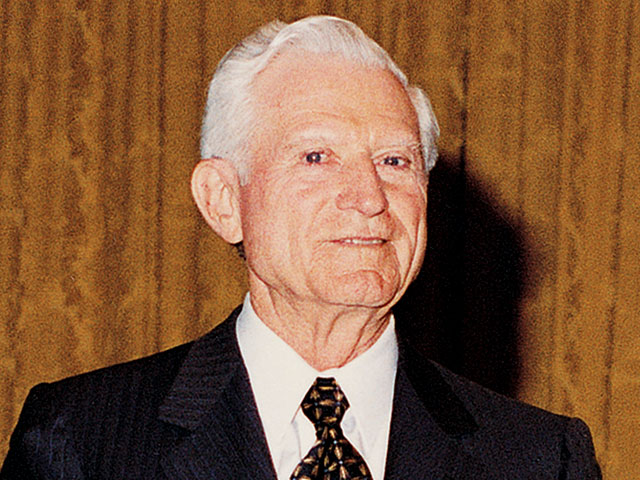
\includegraphics[width=230pt]{fig/amdahl.jpg}
   		\end{center}  
		
  	\end{block}
}
%%%%%%%%%%%%%%%%%%%%%%%%%%%%%%%%%%%%%%%%%%%%%%%%%%%%%%%%%%%%%%%%%%%%%%%%%%%%%%%%%%%%%%%%%


%%%%%%%%%%%%%%%%%%%%%%%%%%%%%%%%%%%%%%%%%%%%%%%%%%%%%%%%%%%%%%%%%%%%%%%%%%%%%%%%%%%%%%%%%%
%%%%%%%%%%%%%%%%%%%%%%%%%%%%%%%%%%%%%%%%%%%%%%%%%%%%%%%%%%%%%%%%%%%%%%%%%%%%%%%%%%%%%%%%%%
\section{Parallel computing}
%%%%%%%%%%%%%%%%%%%%%%%%%%%%%%%%%%%%%%%%%%%%%%%%%%%%%%%%%%%%%%%%%%%%%%%%%%%%%%%%%%%%%%%%%%
%%%%%%%%%%%%%%%%%%%%%%%%%%%%%%%%%%%%%%%%%%%%%%%%%%%%%%%%%%%%%%%%%%%%%%%%%%%%%%%%%%%%%%%%%%

%%%%%%%%%%%%%%%%%%%%%%%%%%%%%%%%%%%%%%%%%%%%%%%%%%%%%%%%%%%%%%%%%%%%%%%%%%%%%%%%%%%%%%%%%%
%%%%%%%%%%%%%%%%%%%%%%%%%%%%%%%%%%%%%%%%%%%%%%%%%%%%%%%%%%%%%%%%%%%%%%%%%%%%%%%%%%%%%%%%%%
\subsection{Key concepts}
%%%%%%%%%%%%%%%%%%%%%%%%%%%%%%%%%%%%%%%%%%%%%%%%%%%%%%%%%%%%%%%%%%%%%%%%%%%%%%%%%%%%%%%%%%

%%%%%%%%%%%%%%%%%%%%%%%%%%%%%%%%%%%%%%%%%%%%%%%%%%%%%%%%%%%%%%%%%%%%%%%%%%%%%%%%%%%%%%%%%%
\frame[t]
{
  \frametitle{Evolution of computing - 1}

      	\begin{center}
 			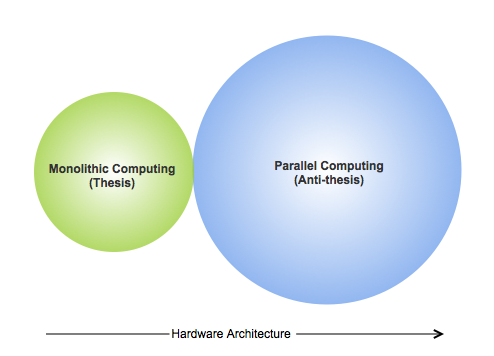
\includegraphics[width=230pt]{fig/hegelian-1.png}
   		\end{center}     

}
%%%%%%%%%%%%%%%%%%%%%%%%%%%%%%%%%%%%%%%%%%%%%%%%%%%%%%%%%%%%%%%%%%%%%%%%%%%%%%%%%%%%%%%%%%


%%%%%%%%%%%%%%%%%%%%%%%%%%%%%%%%%%%%%%%%%%%%%%%%%%%%%%%%%%%%%%%%%%%%%%
\frame[t]
{
  \frametitle{Parallel computing}
    \begin{block}{Background}
      Parallel computing emerged as an anti-thesis.
    	\begin{itemize}
    		\item It is the art of breaking up a big chunk of serial 
    		computation into smaller atomic units which can be done in parallel. 
    		Factors that helped:
		      \begin{itemize}
   		 			\item The arrival of cheap commodity computing hardware.
   		 			\item A theoretical possibility of achieving comparable speeds 
   		 			to serial HPC computing using parallel computing.
					\item Recognition that nature itself is parallel, however complex it may 
					appear. 
			\end{itemize}
		\end{itemize} 
  	\end{block}
}
%%%%%%%%%%%%%%%%%%%%%%%%%%%%%%%%%%%%%%%%%%%%%%%%%%%%%%%%%%%%%%%%%%%%%%%%%%%%%%%%%%%%%%%%%%

%%%%%%%%%%%%%%%%%%%%%%%%%%%%%%%%%%%%%%%%%%%%%%%%%%%%%%%%%%%%%%%%%%%%%%%%%%%%%%%%%%%%%%%%%%
\frame[t]
{
  \frametitle{Parallel computing}
      \begin{block}{Key concepts}
   		\begin{itemize}%[<+-| alert@+>]
			\item A cluster is a network of computers, sometimes called nodes or hosts.
			\item Each computer has several processors.
			\item Each processor has several cores.
			\item A core does the computing.
			\item If an application can use more than one core, it runs faster on a cluster.
   		\end{itemize}
  	\end{block}
}
%%%%%%%%%%%%%%%%%%%%%%%%%%%%%%%%%%%%%%%%%%%%%%%%%%%%%%%%%%%%%%%%%%%%%%%%%%%%%%%%%%%%%%%%%%

%%%%%%%%%%%%%%%%%%%%%%%%%%%%%%%%%%%%%%%%%%%%%%%%%%%%%%%%%%%%%%%%%%%%%%%%%%%%%%%%%%%%%%%%%%
\frame[t]
{
  \frametitle{Parallel computing}
   \begin{block}{Node overview}
   \begin{center}
 		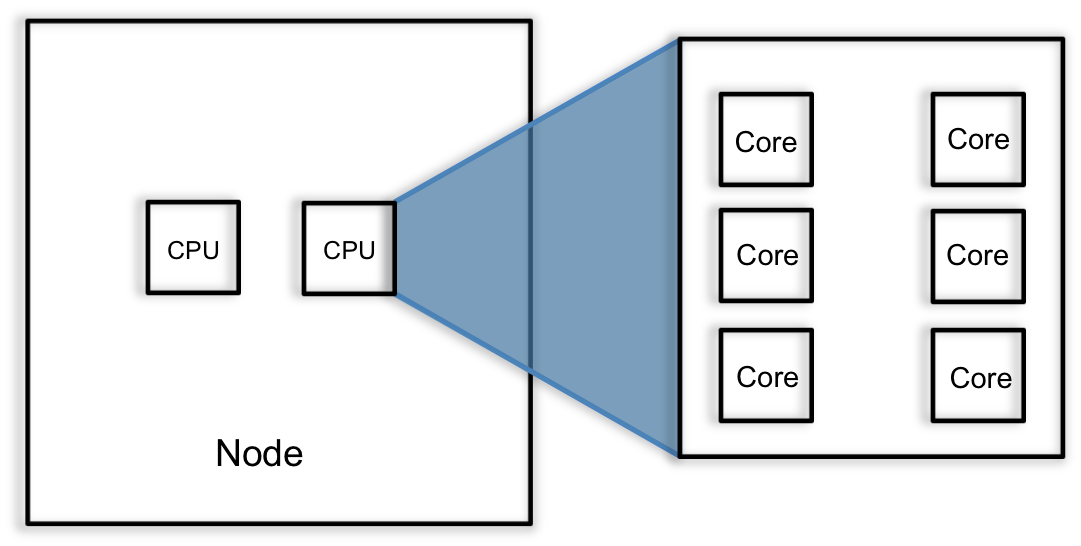
\includegraphics[width=270pt]{NeSI_img/node_view.png}
   	\end{center}
  	\end{block}
}

%%%%%%%%%%%%%%%%%%%%%%%%%%%%%%%%%%%%%%%%%%%%%%%%%%%%%%%%%%%%%%%%%%%%%%%%%%%%%%%%%%%%%%%%%%

%%%%%%%%%%%%%%%%%%%%%%%%%%%%%%%%%%%%%%%%%%%%%%%%%%%%%%%%%%%%%%%%%%%%%%%%%%%%%%%%%%%%%%%%%%
\frame[t]
{
  \frametitle{Parallel computing}
  \framesubtitle{Principles}  
      \begin{itemize}
    	\item Breaking down of a problem into discrete parts that can be solved concurrently.
    	\item Each partial solution consists of a series of instructions.
     	\item Set of instructions are executed simultaneously on different processors.
    \end{itemize}  
          	\begin{center}
 			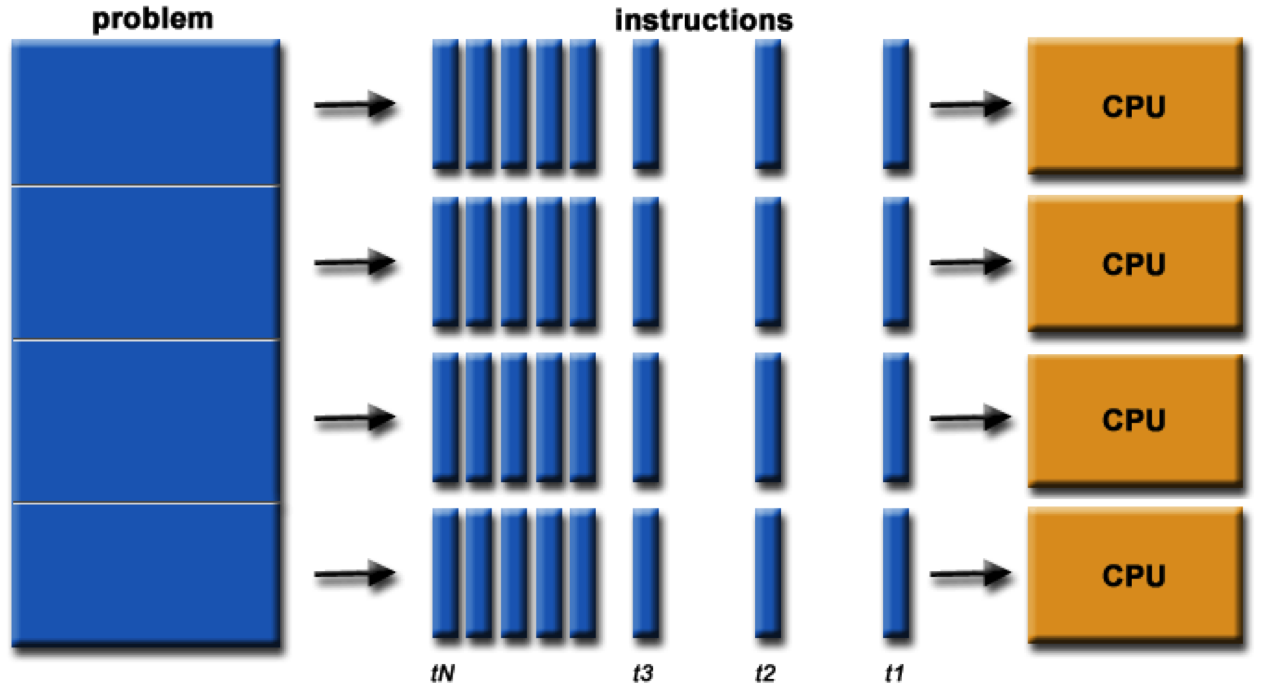
\includegraphics[width=200pt]{fig/parallel-computing.png}
   		\end{center}   
}

%%%%%%%%%%%%%%%%%%%%%%%%%%%%%%%%%%%%%%%%%%%%%%%%%%%%%%%%%%%%%%%%%%%%%%%%%%%%%%%%%%%%%%%%%%

%%%%%%%%%%%%%%%%%%%%%%%%%%%%%%%%%%%%%%%%%%%%%%%%%%%%%%%%%%%%%%%%%%%%%%%%%%%%%%%%%%%%%%%%%%
\frame[t]
{
  \frametitle{Evolution of parallel computing}
     \begin{block}{Grid \& SOA}	      
        \begin{itemize}
           	\item Grid Computing
   			 	\begin{itemize}
   					\item A distributed computing model that orchestrates 
   					computing resources of several academic and research 
   					institutions to work like a unified computing system. 
   			   	\end{itemize}		
   			\item Service Oriented Approach (SOA)
   			 	\begin{itemize}
   					\item In SOA applications are composed by invoking network available 
   					services to accomplish some tasks.
   					\item This paradigm is adopted mainly by business and enterprise community. 
   				\end{itemize}
   		   \end{itemize}
   	\end{block}
}
%%%%%%%%%%%%%%%%%%%%%%%%%%%%%%%%%%%%%%%%%%%%%%%%%%%%%%%%%%%%%%%%%%%%%%%%%%%%%%%%%%%%%%%%%%

%%%%%%%%%%%%%%%%%%%%%%%%%%%%%%%%%%%%%%%%%%%%%%%%%%%%%%%%%%%%%%%%%%%%%%%%%%%%%%%%%%%%%%%%%%
\frame[t]
{
  \frametitle{Evolution of parallel computing}
  \framesubtitle{High performance computing}
        \begin{itemize}
   			\item In 2002, TOP500 list reported that 20 percent of HPC 
			installations as ``clusters''. This marked the emergence of parallel computing
			as a serious platform for HPC.          
			\item By 2013, 80 \% of TOP500 supercomputers were ``clusters''.
        \end{itemize}   		 
   		\begin{center}
 			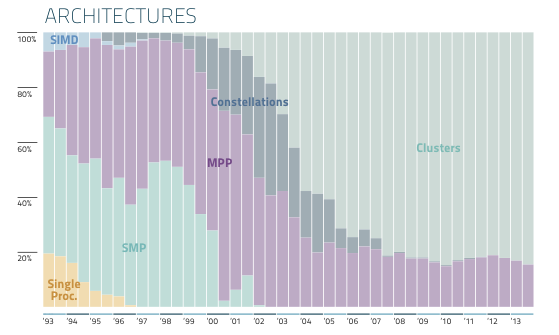
\includegraphics[width=220pt]{fig/TOP50201311_Poster.png}
   		\end{center} 

}
%%%%%%%%%%%%%%%%%%%%%%%%%%%%%%%%%%%%%%%%%%%%%%%%%%%%%%%%%%%%%%%%%%%%%%%%%%%%%%%%%%%%%%%%%%

%%%%%%%%%%%%%%%%%%%%%%%%%%%%%%%%%%%%%%%%%%%%%%%%%%%%%%%%%%%%%%%%%%%%%%%%%%%%%%%%%%%%%%%%%%
\frame[t]
{
  \frametitle{Evolution of computing - 2}

      	\begin{center}
 			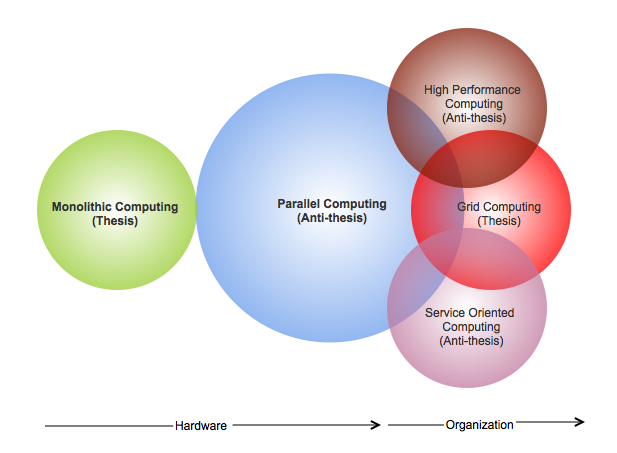
\includegraphics[width=230pt]{fig/hegelian-2.png}
   		\end{center}     

}
%%%%%%%%%%%%%%%%%%%%%%%%%%%%%%%%%%%%%%%%%%%%%%%%%%%%%%%%%%%%%%%%%%%%%%%%%%%%%%%%%%%%%%%%%%

%%%%%%%%%%%%%%%%%%%%%%%%%%%%%%%%%%%%%%%%%%%%%%%%%%%%%%%%%%%%%%%%%%%%%%%%%%%%%%%%%%%%%%%%%%
\frame[t]
{
  \frametitle{Hegelian synthesis}
      \begin{block}{NeSI-like systems}
      	\begin{itemize}
   			\item Mixing grid computing with high performance computing.
   			\item Aiming to cater to research and academic community.
         \end{itemize}
  	\end{block}
    \begin{block}{Cloud providers}
    	\begin{itemize}
   			\item Merging serviced oriented computing with grid concepts.
   			\item Providing services to enterprises and small businesses.
   			    \begin{itemize}
   			    	\item  Orchestrate storage, memory and network resources of 
   			    	geographically distributed data centers as a unified unit.
   			    	\item  The resources are made available to customers on demand with 
   			    	apparent elasticity.
   			    \end{itemize}
         \end{itemize}
  	\end{block}
}
%%%%%%%%%%%%%%%%%%%%%%%%%%%%%%%%%%%%%%%%%%%%%%%%%%%%%%%%%%%%%%%%%%%%%%%%%%%%%%%%%%%%%%%%%%

%%%%%%%%%%%%%%%%%%%%%%%%%%%%%%%%%%%%%%%%%%%%%%%%%%%%%%%%%%%%%%%%%%%%%%%%%%%%%%%%%%%%%%%%%%
%%%%%%%%%%%%%%%%%%%%%%%%%%%%%%%%%%%%%%%%%%%%%%%%%%%%%%%%%%%%%%%%%%%%%%%%%%%%%%%%%%%%%%%%%%
\frame[t]
{
  \frametitle{Evolution of computing - 3}

      	\begin{center}
 			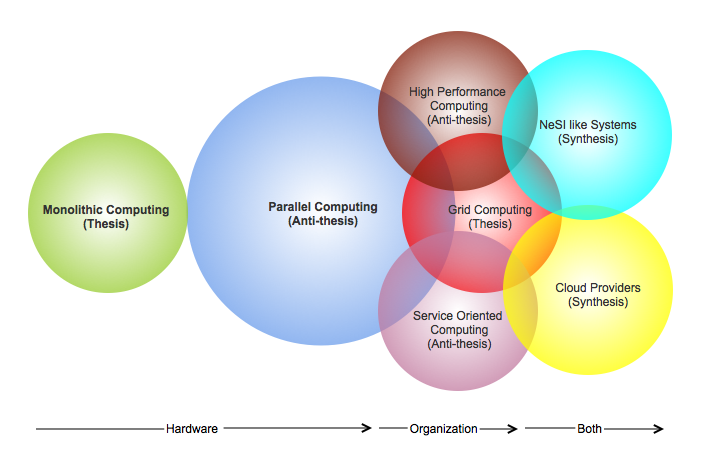
\includegraphics[width=230pt]{fig/hegelian-3.png}
   		\end{center}     
}
%%%%%%%%%%%%%%%%%%%%%%%%%%%%%%%%%%%%%%%%%%%%%%%%%%%%%%%%%%%%%%%%%%%%%%%%%%%%%%%%%%%%%%%%%%

%%%%%%%%%%%%%%%%%%%%%%%%%%%%%%%%%%%%%%%%%%%%%%%%%%%%%%%%%%%%%%%%%%%%%%%%%%%%%%%%%%%%%%%%%%
%\subsection{NeSI Systems}
%%%%%%%%%%%%%%%%%%%%%%%%%%%%%%%%%%%%%%%%%%%%%%%%%%%%%%%%%%%%%%%%%%%%%%%%%%%%%%%%%%%%%%%%%%
%%%%%%%%%%%%%%%%%%%%%%%%%%%%%%%%%%%%%%%%%%%%%%%%%%%%%%%%%%%%%%%%%%%%%%%%%%%%%%%%%%%%%%%%%%

%%%%%%%%%%%%%%%%%%%%%%%%%%%%%%%%%%%%%%%%%%%%%%%%%%%%%%%%%%%%%%%%%%%%%%%%%%%%%%%%%%%%%%%%%%
\frame[t]
{
  \frametitle{NeSI Systems}
      \begin{block}{Facilites}   
      	NeSI HPC resources cater to New Zealand's research and academic community and 
      	are spread between three major facilities:
		\begin{itemize}
			\item BlueFern Supercomputer at the University of Canterbury, Christchurch.
			\item NIWA HPC Facility, Wellington.
			\item Centre for e-Research at the University of Auckland. 
		\end{itemize}	
  There is a single \textbf{grid} interface called \textbf{Grisu} that can be used 
  to access both BlueFern and CeR (NeSI Pan) clusters.
  \end{block}
}
%%%%%%%%%%%%%%%%%%%%%%%%%%%%%%%%%%%%%%%%%%%%%%%%%%%%%%%%%%%%%%%%%%%%%%%%%%%%%%%%%%%%%%%%%%
%%%%%%%%%%%%%%%%%%%%%%%%%%%%%%%%%%%%%%%%%%%%%%%%%%%%%%%%%%%%%%%%%%%%%%%%%%%%%%%%%%%%%%%%%%
\frame[t]
{
  \frametitle{NeSI Systems}
      \begin{block}{Available HPC architectures}
		NeSI provides several kind of HPC architectures and solutions to cater for various needs.
     	\begin{itemize}
     		\item BlueGene/P.
	    	\item Power6 and Power7.
   	    	\item Intel Westmere \& SandyBridge.
			\item Kepler and Fermi GPU servers.
			\item Intel Xeon Phi Co-Processor.
   		\end{itemize}	
  \end{block}
}

%%%%%%%%%%%%%%%%%%%%%%%%%%%%%%%%%%%%%%%%%%%%%%%%%%%%%%%%%%%%%%%%%%%%%%%%%%%%%%%%%%%%%%%%%%



%%%%%%%%%%%%%%%%%%%%%%%%%%%%%%%%%%%%%%%%%%%%%%%%%%%%%%%%%%%%%%%%%%%%%%%%%%%%%%%%%%%%%%%%%%
\frame[t]
{
  \frametitle{NeSI Systems}
      \begin{block}{Available bioinformatics applications}
     	Many general purpose scientific applications are already available in NeSI systems.
     	\begin{itemize}
     		\item \textbf{Velvet:} Sequence assembler for very short reads.
	    	\item \textbf{Bowtie:} Aligns short reads to a reference genome.
   	    	\item \textbf{BLAST:} Searches for regions of similarity between biological sequences.
			\item \textbf{Hmmer:} Protein sequence search and alignment with Hidden Markov Models. 
			\item \textbf{Muscle:} Multiple sequence aligner.
			\item \textbf{PhyML:} Maximum likelihood phylogenies.
			\item \textbf{MrBayes:}  Bayesian inference and model choice across a wide range 
			of phylogenetic and evolutionary models.
   		\end{itemize}	
  \end{block}
}

%%%%%%%%%%%%%%%%%%%%%%%%%%%%%%%%%%%%%%%%%%%%%%%%%%%%%%%%%%%%%%%%%%%%%%%%%%%%%%%%%%%%%%%%%%

%%%%%%%%%%%%%%%%%%%%%%%%%%%%%%%%%%%%%%%%%%%%%%%%%%%%%%%%%%%%%%%%%%%%%%%%%%%%%%%%%%%%%%%%%%
\frame[t]
{
  \frametitle{NeSI Systems: Performance analysis}
  \framesubtitle{PhyML case study: on Pan cluster}

       	\begin{itemize}
     		\item \textbf{PhyML} is a software that estimates maximum likelihood 
     		phylogenies. 
     		\item The right compilers and optimization options for a specific 
     		architecture can increase the performance quite a lot!
     	\end{itemize}
     	\begin{center}
 			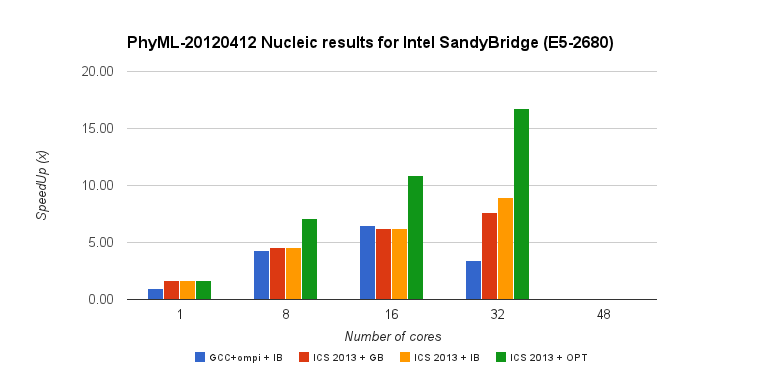
\includegraphics[width=250pt]{fig/speedup-phyml.png}
		\end{center}
}
%%%%%%%%%%%%%%%%%%%%%%%%%%%%%%%%%%%%%%%%%%%%%%%%%%%%%%%%%%%%%%%%%%%%%%%%%%%%%%%%%%%%%%%%%%

%%%%%%%%%%%%%%%%%%%%%%%%%%%%%%%%%%%%%%%%%%%%%%%%%%%%%%%%%%%%%%%%%%%%%%%%%%%%%%%%%%%%%%%%%%
%%%%%%%%%%%%%%%%%%%%%%%%%%%%%%%%%%%%%%%%%%%%%%%%%%%%%%%%%%%%%%%%%%%%%%%%%%%%%%%%%%%%%%%%%%
\section{Parallel programming}
%%%%%%%%%%%%%%%%%%%%%%%%%%%%%%%%%%%%%%%%%%%%%%%%%%%%%%%%%%%%%%%%%%%%%%%%%%%%%%%%%%%%%%%%%%
%%%%%%%%%%%%%%%%%%%%%%%%%%%%%%%%%%%%%%%%%%%%%%%%%%%%%%%%%%%%%%%%%%%%%%%%%%%%%%%%%%%%%%%%%%

%%%%%%%%%%%%%%%%%%%%%%%%%%%%%%%%%%%%%%%%%%%%%%%%%%%%%%%%%%%%%%%%%%%%%%%%%%%%%%%%%%%%%%%%%%
\frame[t]
{
  \frametitle{Parallel programming}
      \begin{block}{Rationale}
		\begin{itemize}
     		\item Is there a rationale for writing your own parallel codes? 
     		\item General purpose scientific applications are good for research. 
     			\begin{itemize}
     				\item Around 80 \% of NeSI cluster usage is by those applications at the moment.
     				\item They are easy to customise and use. 
     			\end{itemize}
     		\item However, as research complexity increases and its scope is refined,
     		general purpose scientific applications may not cater to all the needs of researchers.
     	\end{itemize}
  \end{block}
}
%%%%%%%%%%%%%%%%%%%%%%%%%%%%%%%%%%%%%%%%%%%%%%%%%%%%%%%%%%%%%%%%%%%%%%%%%%%%%%%%%%%%%%%%%%

%%%%%%%%%%%%%%%%%%%%%%%%%%%%%%%%%%%%%%%%%%%%%%%%%%%%%%%%%%%%%%%%%%%%%%%%%%%%%%%%%%%%%%%%%%
\frame[t]
{
  \frametitle{Parallel problems}
  \framesubtitle{Case Study: N Body Problem} 
  	\begin{center} 
      	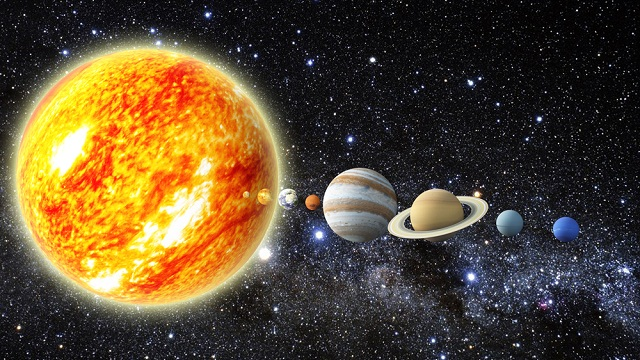
\includegraphics[width=230pt]{fig/solar-system.jpg}	
	\end{center}  
	\begin{center}  
		Gravitational n-body problem (Newton's laws of force) \\
		Force is a function of mass and acceleration ($f = m \times a$)
	\end{center}  
}
%%%%%%%%%%%%%%%%%%%%%%%%%%%%%%%%%%%%%%%%%%%%%%%%%%%%%%%%%%%%%%%%%%%%%%%%%%%%%%%%%%%%%%%%%%

%%%%%%%%%%%%%%%%%%%%%%%%%%%%%%%%%%%%%%%%%%%%%%%%%%%%%%%%%%%%%%%%%%%%%%%%%%%%%%%%%%%%%%%%%%
\frame[t]
{
  \frametitle{Parallel programming}
  \framesubtitle{Case Study: N Body Problem}
    	\begin{figure}
   			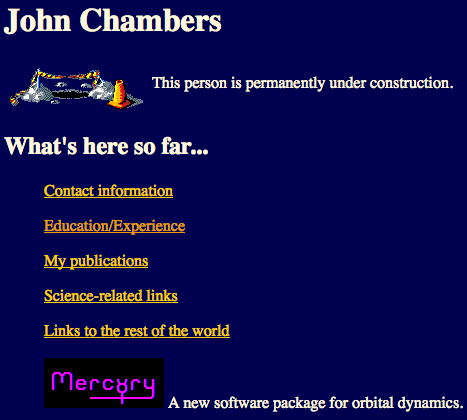
\includegraphics[width=0.45\textwidth]{fig/john-chambers.png}
   			\hfill
   			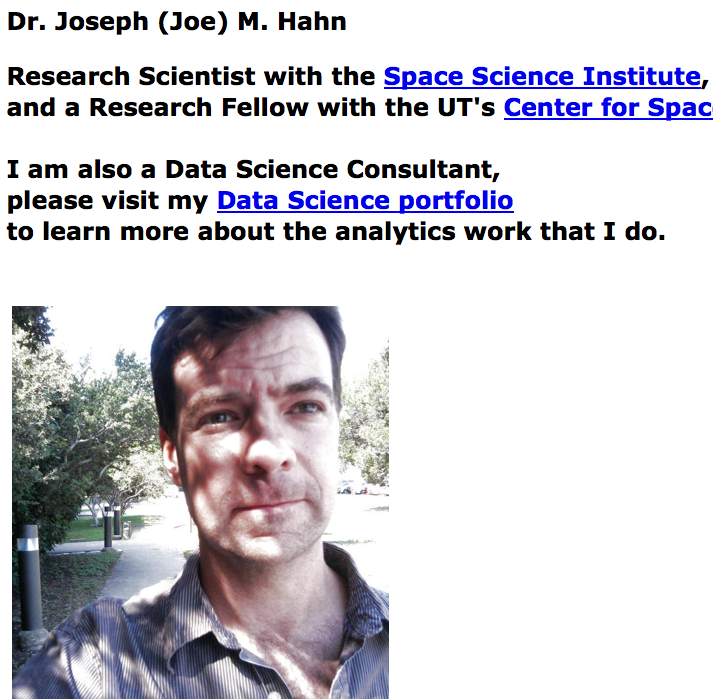
\includegraphics[width=0.40\textwidth]{fig/joseph-hahn.png}
      	\end{figure}  
	\begin{itemize}
     		\item Mercury: N body simulator developed
     		by  Dr John Chamber at NASA Ames Research Center, California
     		\item Dr Joseph M. Hahn of Space Science Institute, Colorado had to come up with a 
     		variant Mercury to take care of additional drag forces that drive planet migration!
    \end{itemize}    		

}
%%%%%%%%%%%%%%%%%%%%%%%%%%%%%%%%%%%%%%%%%%%%%%%%%%%%%%%%%%%%%%%%%%%%%%%%%%%%%%%%%%%%%%%%%%


%%%%%%%%%%%%%%%%%%%%%%%%%%%%%%%%%%%%%%%%%%%%%%%%%%%%%%%%%%%%%%%%%%%%%%%%%%%%%%%%%%%%%%%%%%
\frame[t]
{
  \frametitle{Parallel programming}
  \framesubtitle{Case Study: N Body Problem}
      
    	\begin{center}
   			
\includegraphics[width=180pt]{fig/philip-sharp.png}
      	\end{center} 
      	
		\begin{itemize}
     		\item Philip Sharp at University of Auckland started 
     		implementing Mercury n-body integration on GPUs.
     		\item Then he found out that he has been experimenting with more robust 
     		versions of those techniques.
     		\item He is now rebuilding the n-body integrator from scratch. 
     	\end{itemize}

}
%%%%%%%%%%%%%%%%%%%%%%%%%%%%%%%%%%%%%%%%%%%%%%%%%%%%%%%%%%%%%%%%%%%%%%%%%%%%%%%%%%%%%%%%%%

%%%%%%%%%%%%%%%%%%%%%%%%%%%%%%%%%%%%%%%%%%%%%%%%%%%%%%%%%%%%%%%%%%%%%%%%%%%%%%%%%%%%%%%%%%
%%%%%%%%%%%%%%%%%%%%%%%%%%%%%%%%%%%%%%%%%%%%%%%%%%%%%%%%%%%%%%%%%%%%%%%%%%%%%%%%%%%%%%%%%%
\subsection{Parallel decomposition}
%%%%%%%%%%%%%%%%%%%%%%%%%%%%%%%%%%%%%%%%%%%%%%%%%%%%%%%%%%%%%%%%%%%%%%%%%%%%%%%%%%%%%%%%%%
%%%%%%%%%%%%%%%%%%%%%%%%%%%%%%%%%%%%%%%%%%%%%%%%%%%%%%%%%%%%%%%%%%%%%%%%%%%%%%%%%%%%%%%%%%


%%%%%%%%%%%%%%%%%%%%%%%%%%%%%%%%%%%%%%%%%%%%%%%%%%%%%%%%%%%%%%%%%%%%%%%%%%%%%%%%%%%%%%%%%%
%%%%%%%%%%%%%%%%%%%%%%%%%%%%%%%%%%%%%%%%%%%%%%%%%%%%%%%%%%%%%%%%%%%%%%%%%%%%%%%%%%%%%%%%%%
\subsubsection{N body problem}
%%%%%%%%%%%%%%%%%%%%%%%%%%%%%%%%%%%%%%%%%%%%%%%%%%%%%%%%%%%%%%%%%%%%%%%%%%%%%%%%%%%%%%%%%%
%%%%%%%%%%%%%%%%%%%%%%%%%%%%%%%%%%%%%%%%%%%%%%%%%%%%%%%%%%%%%%%%%%%%%%%%%%%%%%%%%%%%%%%%%%

%%%%%%%%%%%%%%%%%%%%%%%%%%%%%%%%%%%%%%%%%%%%%%%%%%%%%%%%%%%%%%%%%%%%%%%%%%%%%%%%%%%%%%%%%%
\frame[t]
{
  \frametitle{Parallel programming}
    \framesubtitle{Case Study: N Body Problem}
    We need to look for hotspots and bottlenecks to parallelise an algorithm. 
      \begin{block}{Hotspots}
      	
		\begin{itemize}  
     		\item Hotspots are the areas where we have massive iterative works, which 
     		can be parallelized into smaller units that are 
     		independent of each other. 
     		\item Those units of work are called tasks and such algorithms are often described
     		as ``embarrassingly parallel''.
      	\end{itemize}
   
  \end{block}
}
%%%%%%%%%%%%%%%%%%%%%%%%%%%%%%%%%%%%%%%%%%%%%%%%%%%%%%%%%%%%%%%%%%%%%%%%%%%%%%%%%%%%%%%%%%

%%%%%%%%%%%%%%%%%%%%%%%%%%%%%%%%%%%%%%%%%%%%%%%%%%%%%%%%%%%%%%%%%%%%%%%%%%%%%%%%%%%%%%%%%%
\frame[t]
{
  \frametitle{Parallel programming}
    \framesubtitle{Case Study: N Body Problem}
      \begin{block}{Bottlenecks}
      	
		\begin{itemize}  
     		\item Bottlenecks are the places where computations become inter-dependent. 
     		Usually there is a need to synchronise the data before we 
     		begin another set of parallel tasks. 
     		\item If an algorithm has got too many inter-dependent tasks, it will be called
     		a fine-grained algorithm, and may not able to parallelise efficiently. 
      	\end{itemize}
   
  \end{block}
}
%%%%%%%%%%%%%%%%%%%%%%%%%%%%%%%%%%%%%%%%%%%%%%%%%%%%%%%%%%%%%%%%%%%%%%%%%%%%%%%%%%%%%%%%%%


%%%%%%%%%%%%%%%%%%%%%%%%%%%%%%%%%%%%%%%%%%%%%%%%%%%%%%%%%%%%%%%%%%%%%%%%%%%%%%%%%%%%%%%%%%
\begin{frame}{Direct n-body problem}
  \framesubtitle{Governing equations}
	\begin{equation}
	\textbf{f}_{ij} = G \frac{m_i m_j}{||\textbf{r}_{ij}||^2} \cdot \frac{\textbf{r}_{ij}}{||\textbf{r}_{ij}||}
	\end{equation}
	\begin{equation}
	\textbf{F}_i = \sum_{1 \le j \le N} \textbf{f}_{ij} \;\; ,\; j \ne i
	\end{equation}
	\begin{equation}
	\textbf{F}_i = m_i \textbf{a}_i
	\end{equation}
	\begin{equation}
	\textbf{p}_i = \iint \textbf{a}_i\,\textrm{d}t
	\end{equation}
Where:
	\begin{itemize}
	 	\item Force (F) is a function of mass and acceleration (2).
	 	\item Position (p) is a function of velocity/acceleration and time (4).
	\end{itemize}	 	
	
\end{frame}
%%%%%%%%%%%%%%%%%%%%%%%%%%%%%%%%%%%%%%%%%%%%%%%%%%%%%%%%%%%%%%%%%%%%%%%%%%%%%%%%%%%%%%%%%%

%%%%%%%%%%%%%%%%%%%%%%%%%%%%%%%%%%%%%%%%%%%%%%%%%%%%%%%%%%%%%%%%%%%%%%%%%%%%%%%%%%%%%%%%%%

\begin{frame}[fragile]
\frametitle{Direct n-body problem}
  \framesubtitle{Pseudocode}
	\begin{algorithm}[H]
	\begin{algorithmic}[1]


\STATE Input initial positons and velocities of particles
\WHILE {each simulation step}
	\FOR {each particle}\\
		\STATE Compute total force on the particle \\
	\ENDFOR
	
	\FOR {each particle}
		\STATE Compute velocity and position of the particle\\
	\ENDFOR	
\STATE  Output new velocity and position of particles\\
\ENDWHILE
\STATE  Output final velocity and position of particles\\

\end{algorithmic}
%\caption{Pseudocode for N body problem }
\label{alg:seq}
\end{algorithm}
\end{frame}


%%%%%%%%%%%%%%%%%%%%%%%%%%%%%%%%%%%%%%%%%%%%%%%%%%%%%%%%%%%%%%%%%%%%%%%%%%%%%%%%%%%%%%%%%%


%%%%%%%%%%%%%%%%%%%%%%%%%%%%%%%%%%%%%%%%%%%%%%%%%%%%%%%%%%%%%%%%%%%%%%%%%%%%%%%%%%%%%%%%%%
\frame[t]
{
  \frametitle{Direct n-body problem}
      \begin{block}{Parallel decomposition}
      There are two major decomposition techniques:
      	\begin{itemize}
      	\item Domain/data decomposition
		  \begin{itemize}
				\item Forms the foundation for most parallel algorithms 
				\item Here we assign different subset of data to different processors
				and do the same or similar computation over them. 
			\end{itemize}
      	\item Functional/task decomposition
		  \begin{itemize}
				\item An alternative strategy where we assign different 
				functions to different processors.
				\item When algorithms have no obvious data structure that can be decomposed.
				\item It could be the case of a single task at the root of a 
				tree creates new tasks for each subtree, based on the mode of computation
				rather than the structure of the data.
			\end{itemize}
      	\end{itemize}
   
  \end{block}
}
%%%%%%%%%%%%%%%%%%%%%%%%%%%%%%%%%%%%%%%%%%%%%%%%%%%%%%%%%%%%%%%%%%%%%%%%%%%%%%%%%%%%%%%%%%

%%%%%%%%%%%%%%%%%%%%%%%%%%%%%%%%%%%%%%%%%%%%%%%%%%%%%%%%%%%%%%%%%%%%%%%%%%%%%%%%%%%%%%%%%%
%%%%%%%%%%%%%%%%%%%%%%%%%%%%%%%%%%%%%%%%%%%%%%%%%%%%%%%%%%%%%%%%%%%%%%%%%%%%%%%%%%%%%%%%%%
%\subsubsection{Data decomposition}
%%%%%%%%%%%%%%%%%%%%%%%%%%%%%%%%%%%%%%%%%%%%%%%%%%%%%%%%%%%%%%%%%%%%%%%%%%%%%%%%%%%%%%%%%%
%%%%%%%%%%%%%%%%%%%%%%%%%%%%%%%%%%%%%%%%%%%%%%%%%%%%%%%%%%%%%%%%%%%%%%%%%%%%%%%%%%%%%%%%%%

%%%%%%%%%%%%%%%%%%%%%%%%%%%%%%%%%%%%%%%%%%%%%%%%%%%%%%%%%%%%%%%%%%%%%%%%%%%%%%%%%%%%%%%%%%
\frame[t]
{
  \frametitle{Direct n-body problem}
      \begin{block}{Parallel decomposition}
      		\begin{itemize}
				\item We can visualize bodies in direct n-body problem as elements of 
				 an array.
				\item This data can be divided into subsets: it is a case of domain/data
				parallelism.

			\end{itemize}
   
  \end{block}
}
%%%%%%%%%%%%%%%%%%%%%%%%%%%%%%%%%%%%%%%%%%%%%%%%%%%%%%%%%%%%%%%%%%%%%%%%%%%%%%%%%%%%%%%%%

%%%%%%%%%%%%%%%%%%%%%%%%%%%%%%%%%%%%%%%%%%%%%%%%%%%%%%%%%%%%%%%%%%%%%%%%%%%%%%%%%%%%%%%


%%%%%%%%%%%%%%%%%%%%%%%%%%%%%%%%%%%%%%%%%%%%%%%%%%%%%%%%%%%%%%%%%%%%%%%%%%%%%%%%%%%%%%%%%%
\frame[t]
{
  \frametitle{Direct n-body problem}
      \begin{block}{Data decomposition as an array}
        \begin{figure}
   			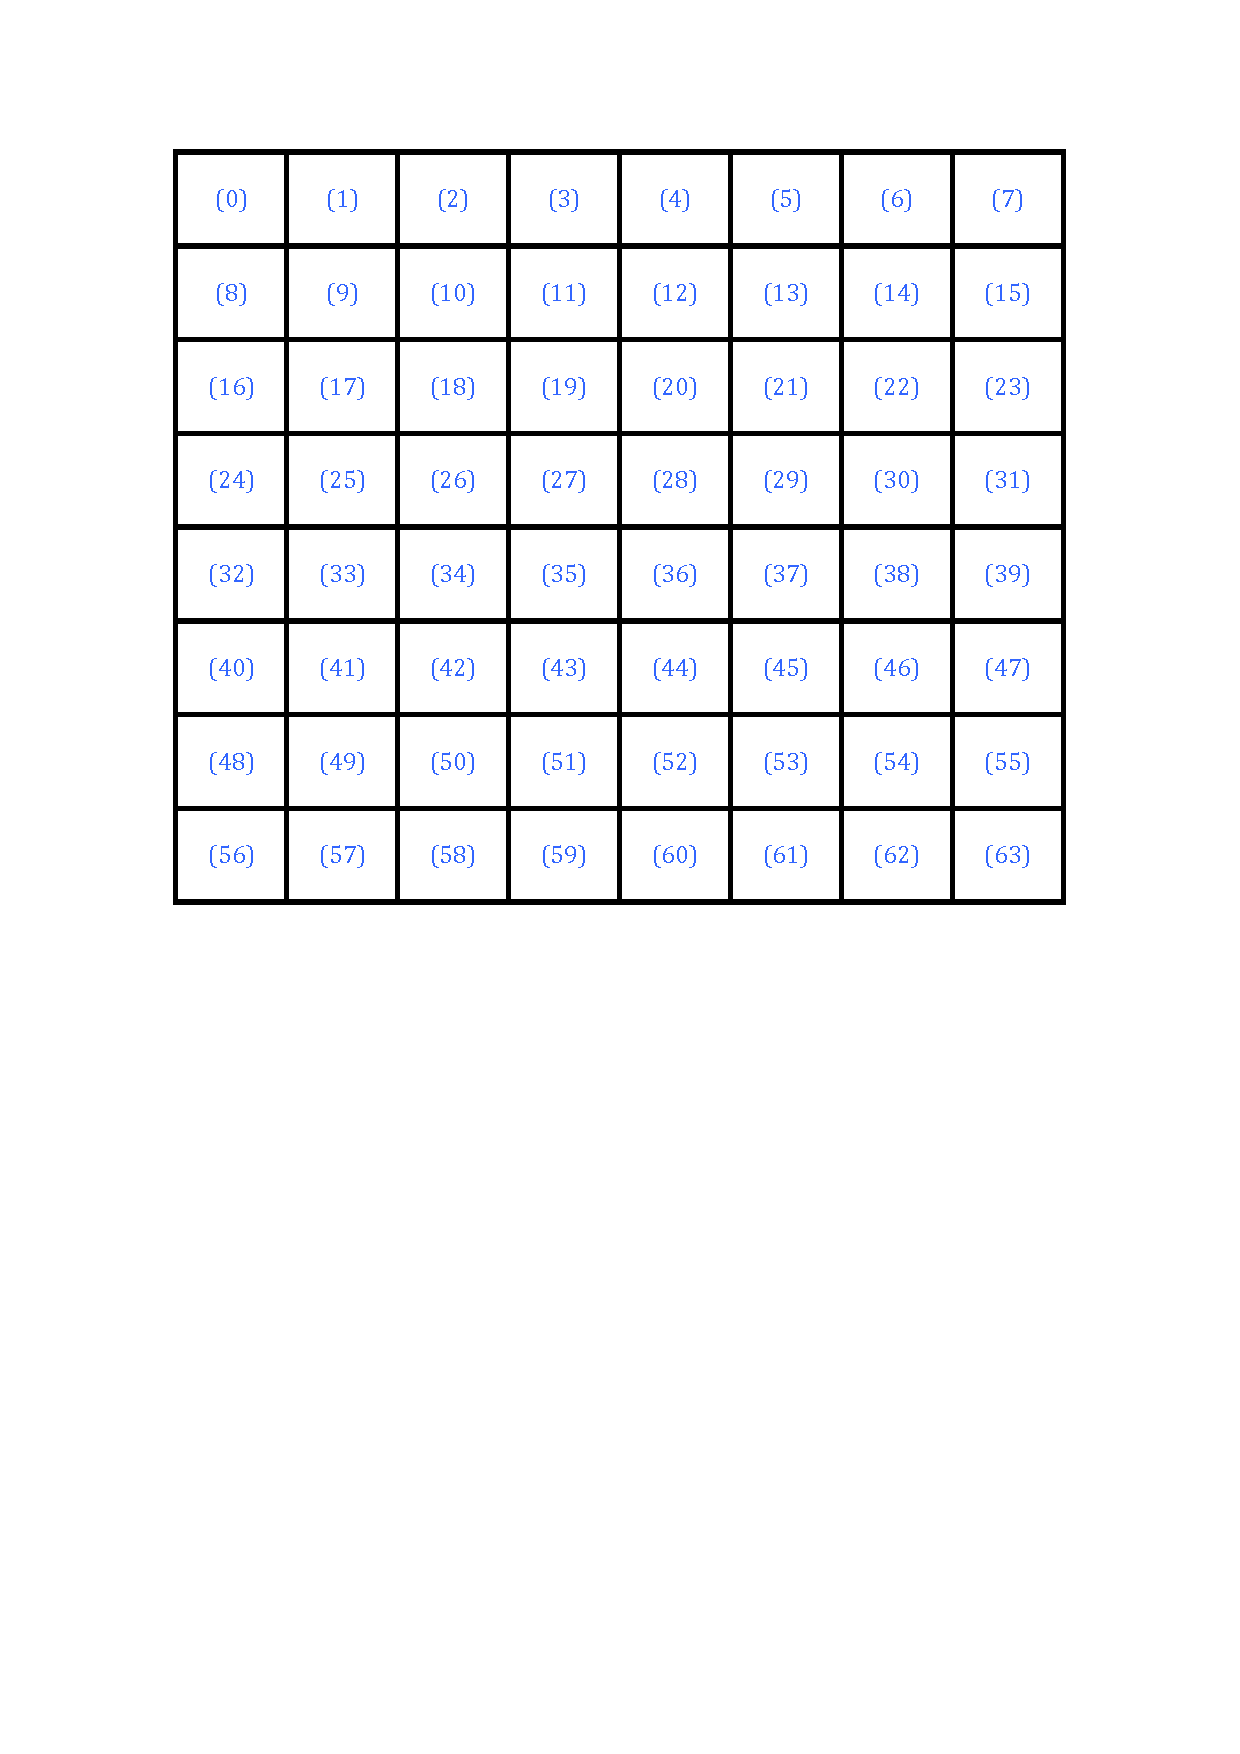
\includegraphics[width=0.475\textwidth]{fig/grid-1d.pdf}
   			\hfill
   			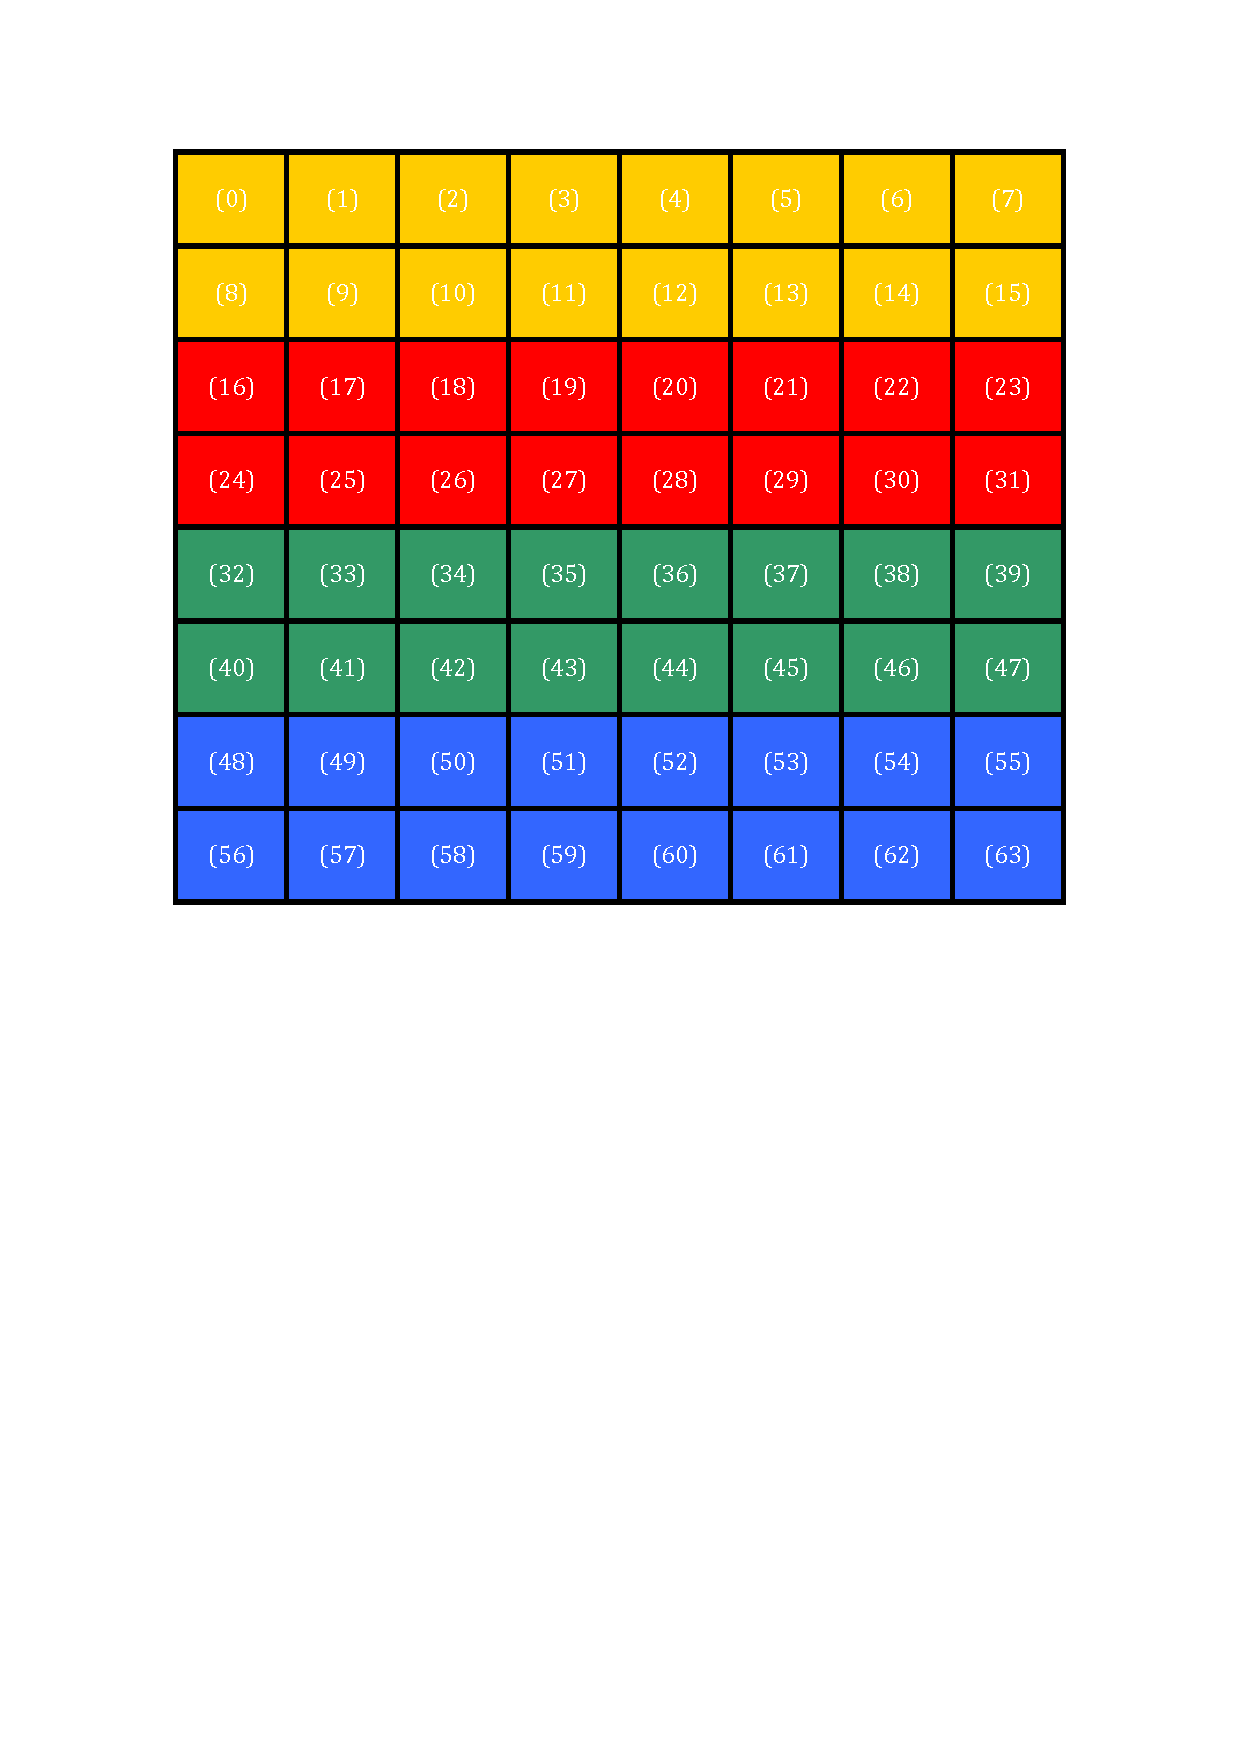
\includegraphics[width=0.475\textwidth]{fig/grid-1d-decomp.pdf}
      	\end{figure}   
  \end{block}
}
%%%%%%%%%%%%%%%%%%%%%%%%%%%%%%%%%%%%%%%%%%%%%%%%%%%%%%%%%%%%%%%%%%%%%%%%%%%%%%%%%%%%%%%%%%

%%%%%%%%%%%%%%%%%%%%%%%%%%%%%%%%%%%%%%%%%%%%%%%%%%%%%%%%%%%%%%%%%%%%%%%%%%%%%%%%%%%%%%%%%%
\frame[t]
{
  \frametitle{Direct n-body problem}
      \begin{block}{Data decomposition as a matrix}
    	\begin{figure}
   			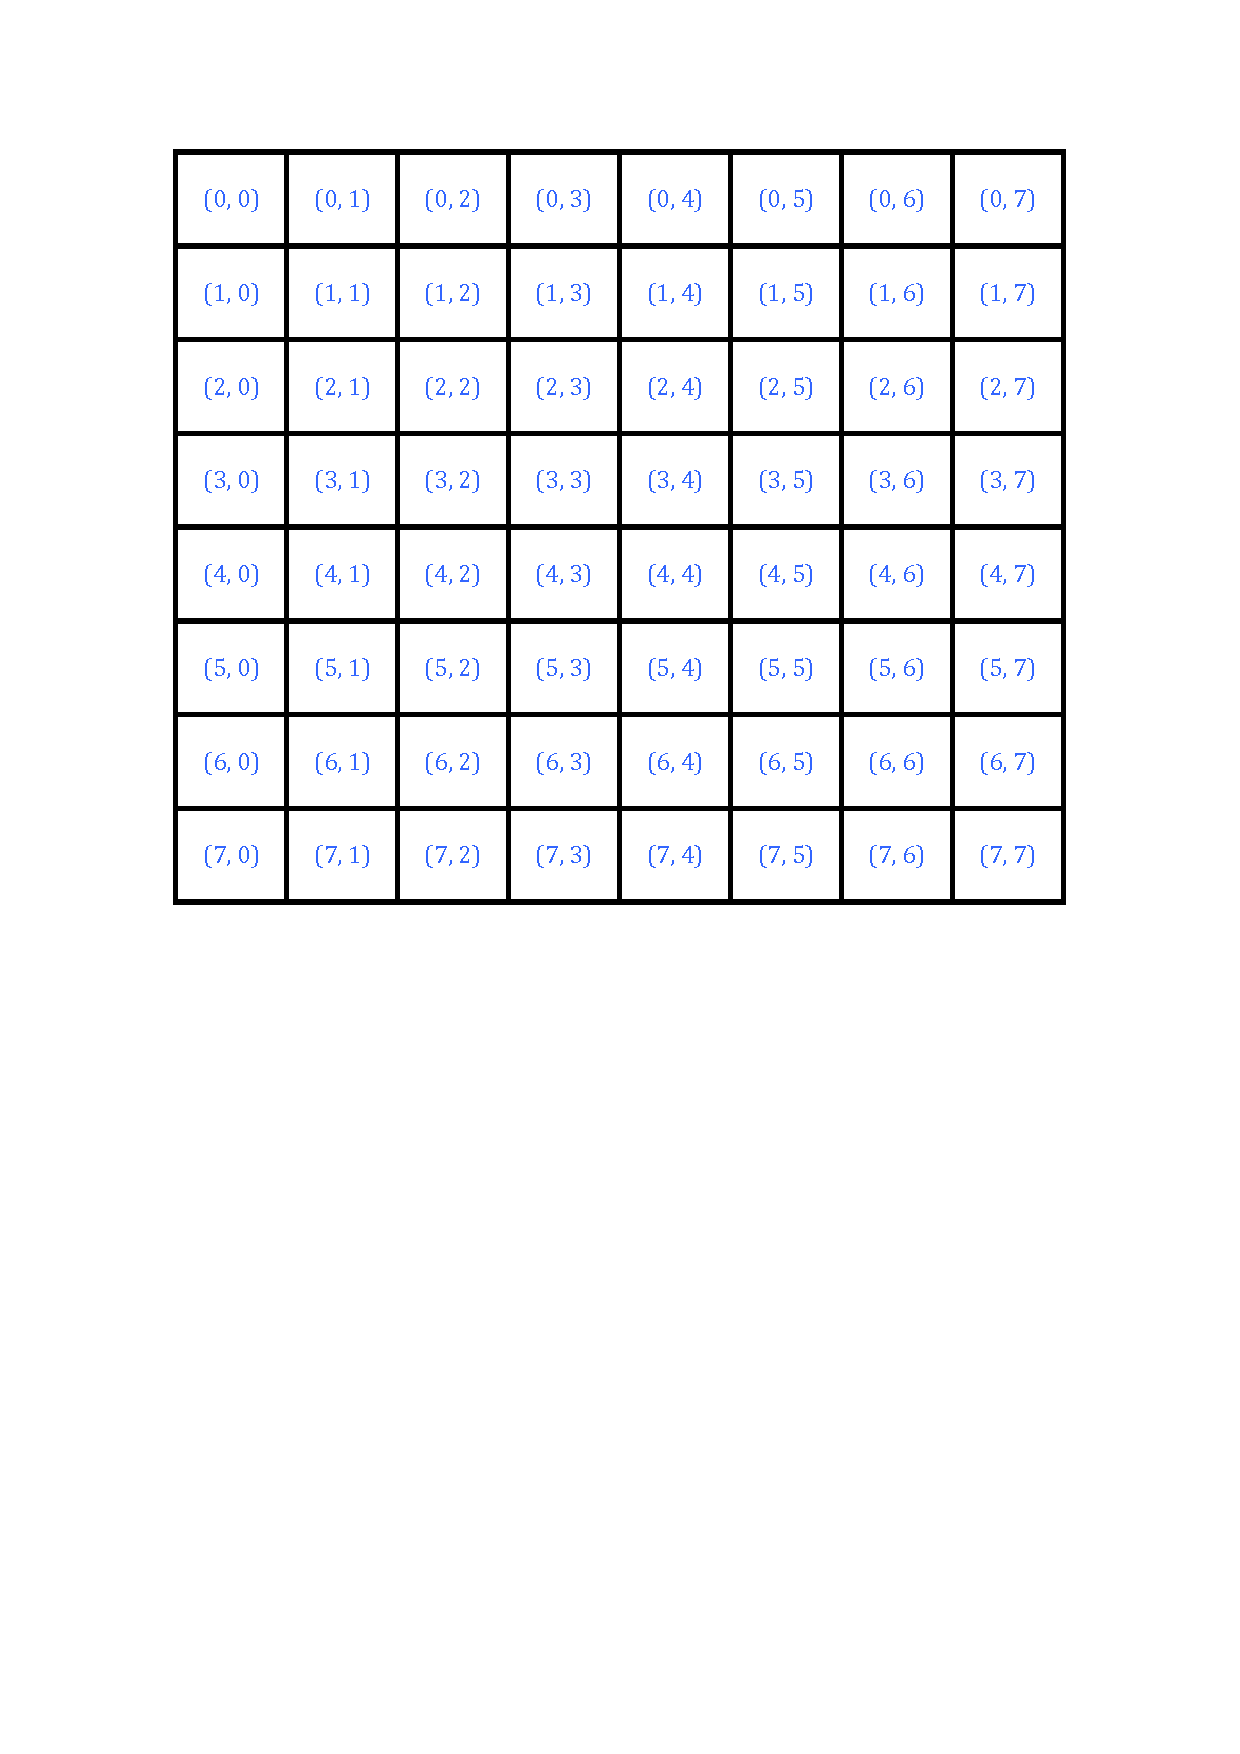
\includegraphics[width=0.475\textwidth]{fig/grid-2d.pdf}
   			\hfill
   			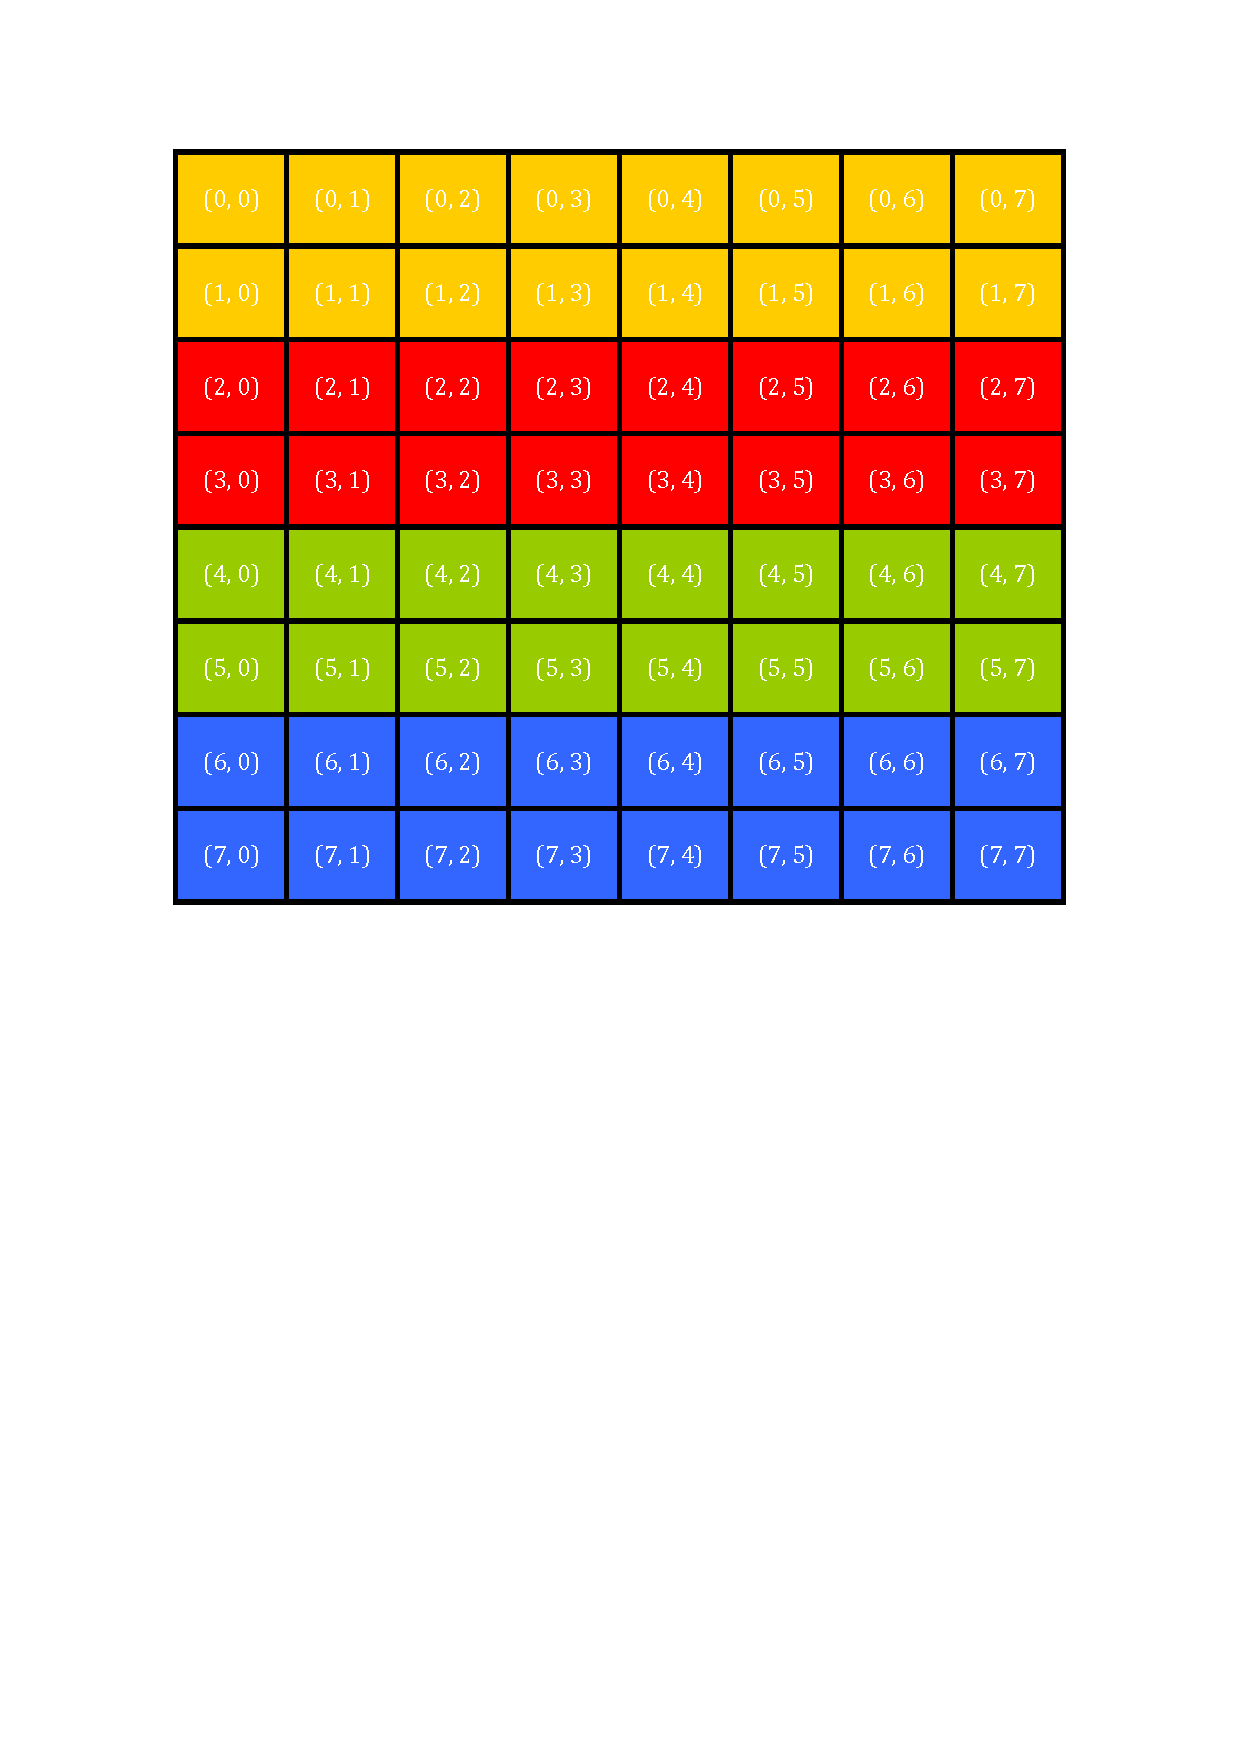
\includegraphics[width=0.475\textwidth]{fig/grid-2d-decomp.pdf}
      	\end{figure}      
  \end{block}
}
%%%%%%%%%%%%%%%%%%%%%%%%%%%%%%%%%%%%%%%%%%%%%%%%%%%%%%%%%%%%%%%%%%%%%%%%%%%%%%%%%%%%%%%%%%

%%%%%%%%%%%%%%%%%%%%%%%%%%%%%%%%%%%%%%%%%%%%%%%%%%%%%%%%%%%%%%%%%%%%%%%%%%%%%%%%%%%%%%%%%%
\frame[t]
{
  \frametitle{Direct n-body problem}
      \begin{block}{Parallel decomposition}
      		\begin{itemize}
      			\item The algorithm is reduced to parallel matrix-vector operations.
				\item However, all nodes need to have access to all the data in this model,
				which could put constraints on memory.
				\item There are other n-body algorithms to mitigate this issue, where 
				bodies are geographically grouped together and considered as a large 
				single body (Example: Barnes–Hut method).
			\end{itemize}
   
  \end{block}
}
%%%%%%%%%%%%%%%%%%%%%%%%%%%%%%%%%%%%%%%%%%%%%%%%%%%%%%%%%%%%%%%%%%%%%%%%%%%%%%%%%%%%%%%%%

%%%%%%%%%%%%%%%%%%%%%%%%%%%%%%%%%%%%%%%%%%%%%%%%%%%%%%%%%%%%%%%%%%%%%%%%%%%%%%%%%%%%%%%%%%
\frame[t]
{
  \frametitle{N-body problem}
    \begin{block}{Barnes–Hut method}
         \begin{center}
 			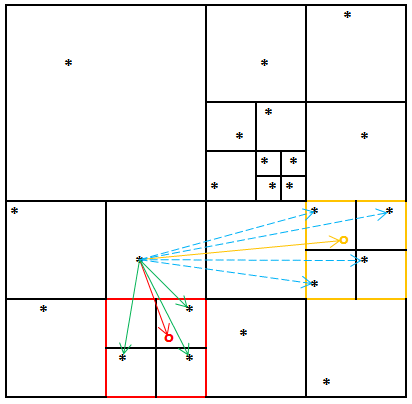
\includegraphics[width=130pt]{fig/barnes-hut.png}
   		 \end{center} 
   	Technically, it reduces the complexity of problem from $O(n^2)$to $O(n \times log n)$
   	\end{block} 
}
%%%%%%%%%%%%%%%%%%%%%%%%%%%%%%%%%%%%%%%%%%%%%%%%%%%%%%%%%%%%%%%%%%%%%%%%%%%%%%%%%%%%%%%%%%



%%%%%%%%%%%%%%%%%%%%%%%%%%%%%%%%%%%%%%%%%%%%%%%%%%%%%%%%%%%%%%%%%%%%%%%%%%%%%%%%%%%%%%%%%%
\frame[t]
{
  \frametitle{Parallel decomposition}
  	\framesubtitle{Heat diffusion problem}
      \begin{figure}%[htb]
         \begin{center}
 			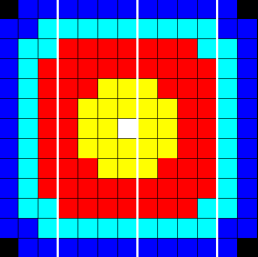
\includegraphics[width=150pt]{fig/heat-diffusion-llnl.png}\\
   			\caption {Heat diffusion on a 2D plate}  
   		 \end{center}  
   		 Crux: To update each cell, we need information about all its neighbouring cells. 
   	 \end{figure}
}
%%%%%%%%%%%%%%%%%%%%%%%%%%%%%%%%%%%%%%%%%%%%%%%%%%%%%%%%%%%%%%%%%%%%%%%%%%%%%%%%%%%%%%%%%%


%%%%%%%%%%%%%%%%%%%%%%%%%%%%%%%%%%%%%%%%%%%%%%%%%%%%%%%%%%%%%%%%%%%%%%%%%%%%%%%%%%%%%%%%%%
\frame[t]
{
  \frametitle{Parallel decomposition}
  	\framesubtitle{Heat diffusion problem}
      \begin{block}{The economy of decomposition}
    	\begin{figure}
   			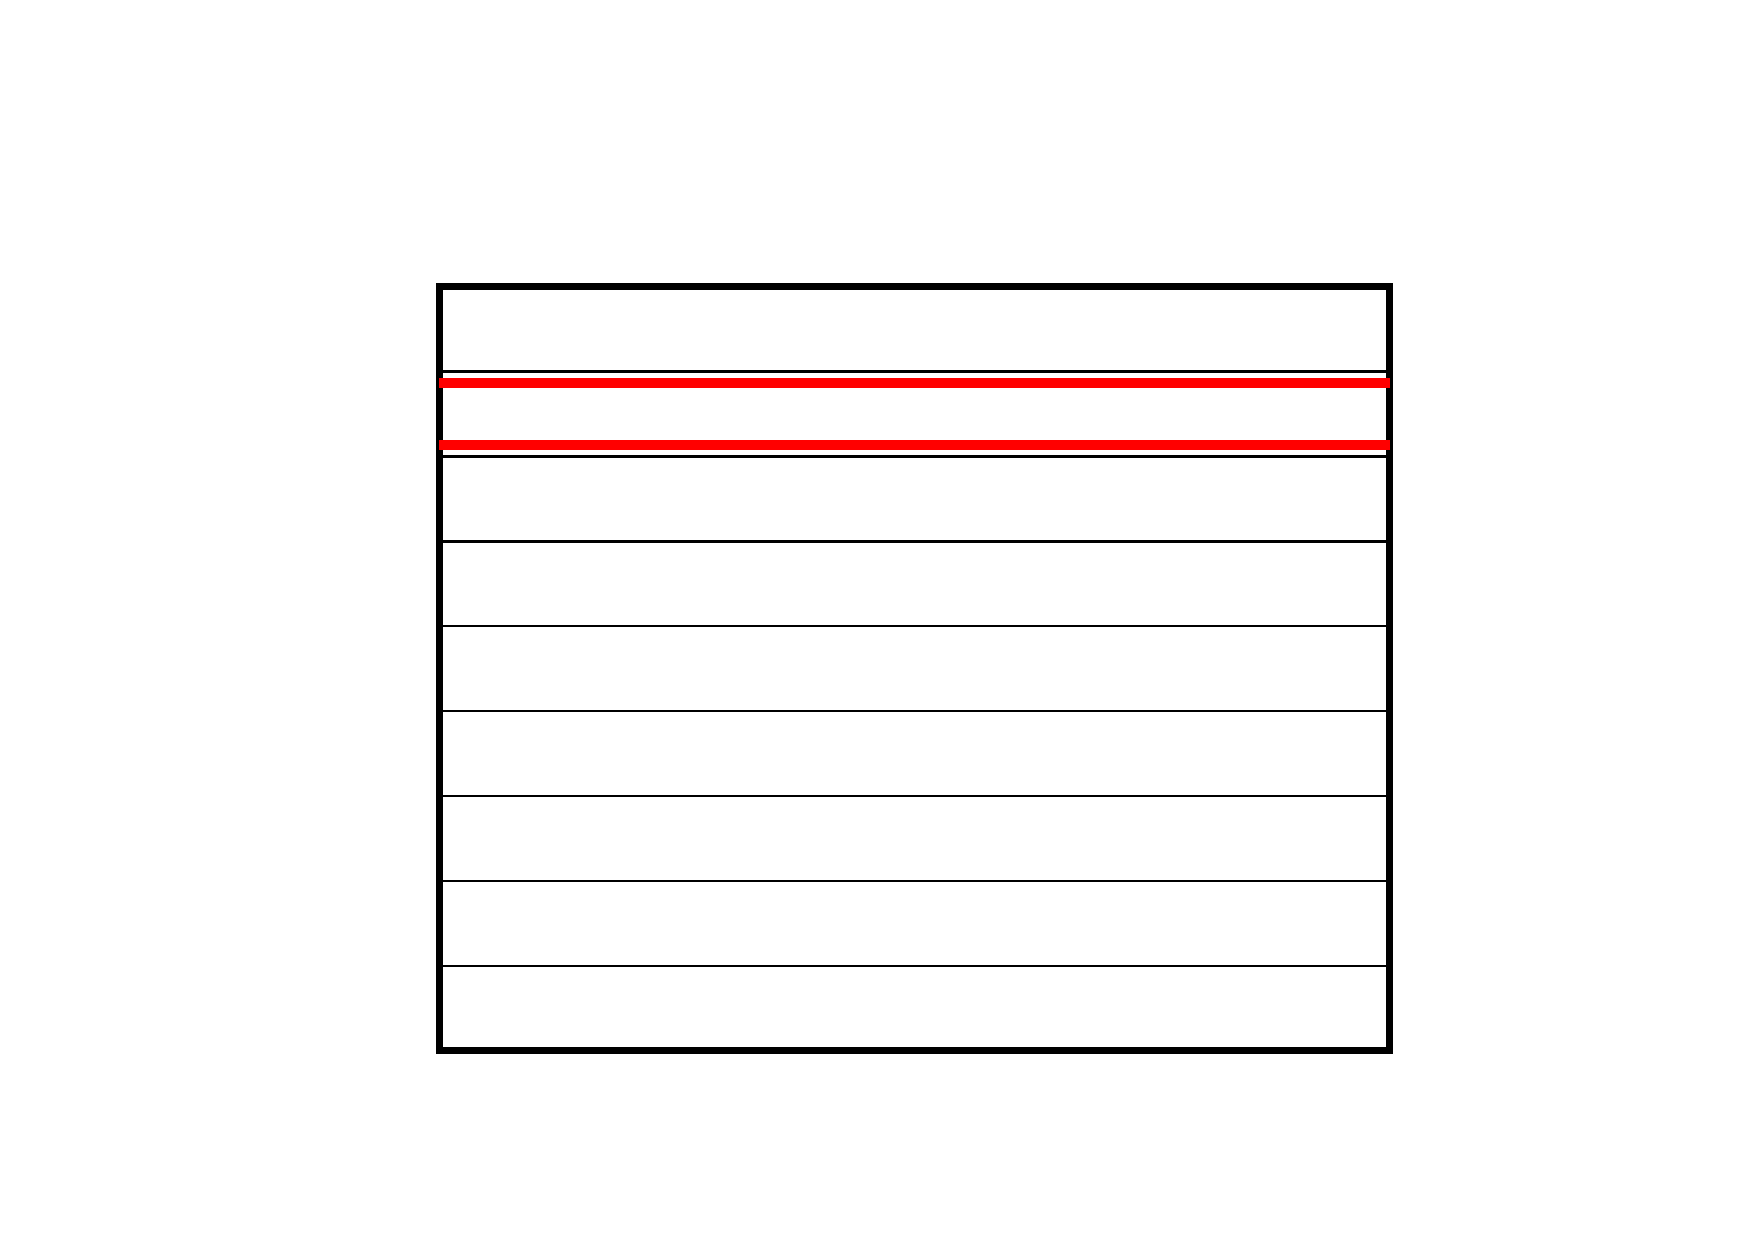
\includegraphics[width=0.37\textwidth]{fig/ht-row.pdf}
   			\hfill
   			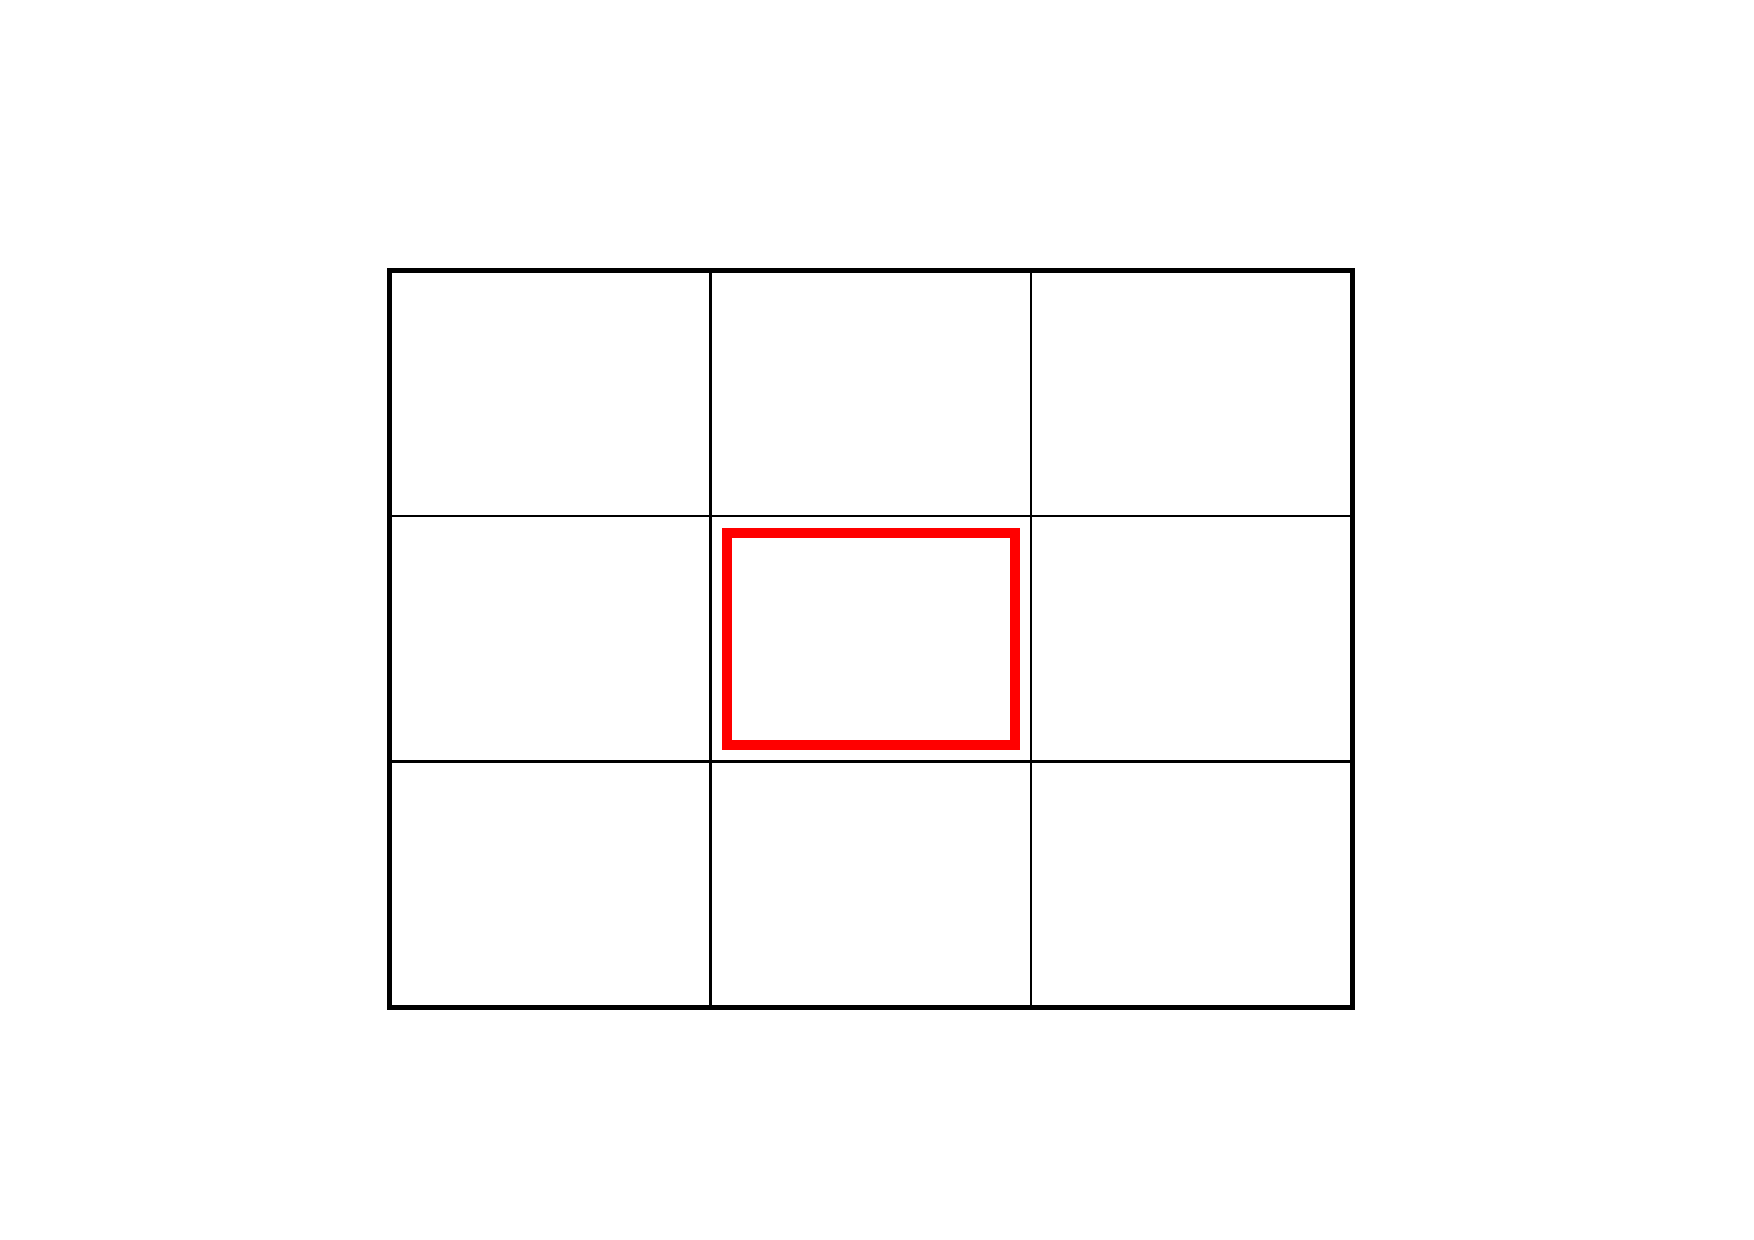
\includegraphics[width=0.37\textwidth]{fig/ht-cube.pdf}
      	\end{figure}
      	Partitioning as near-square rectangular blocks 
      	will give an advantage of $4\times (\sqrt{p}$ - $1)N/\sqrt{p}$ times over 
      	partitioning as rows (where $p$ is total perimeter and $N$ is number of partitions) 
      	in terms of the amount of data to be synchronized.     
  \end{block}
}
%%%%%%%%%%%%%%%%%%%%%%%%%%%%%%%%%%%%%%%%%%%%%%%%%%%%%%%%%%%%%%%%%%%%%%%%%%%%%%%%%%%%%%%%%%

%%%%%%%%%%%%%%%%%%%%%%%%%%%%%%%%%%%%%%%%%%%%%%%%%%%%%%%%%%%%%%%%%%%%%%%%%%%%%%%%%%%%%%%%%%
\frame[t]
{
  \frametitle{Parallel decomposition}
  	\framesubtitle{Heat diffusion problem}
      \begin{block}{Ghost cells}
      
      \begin{figure}
   		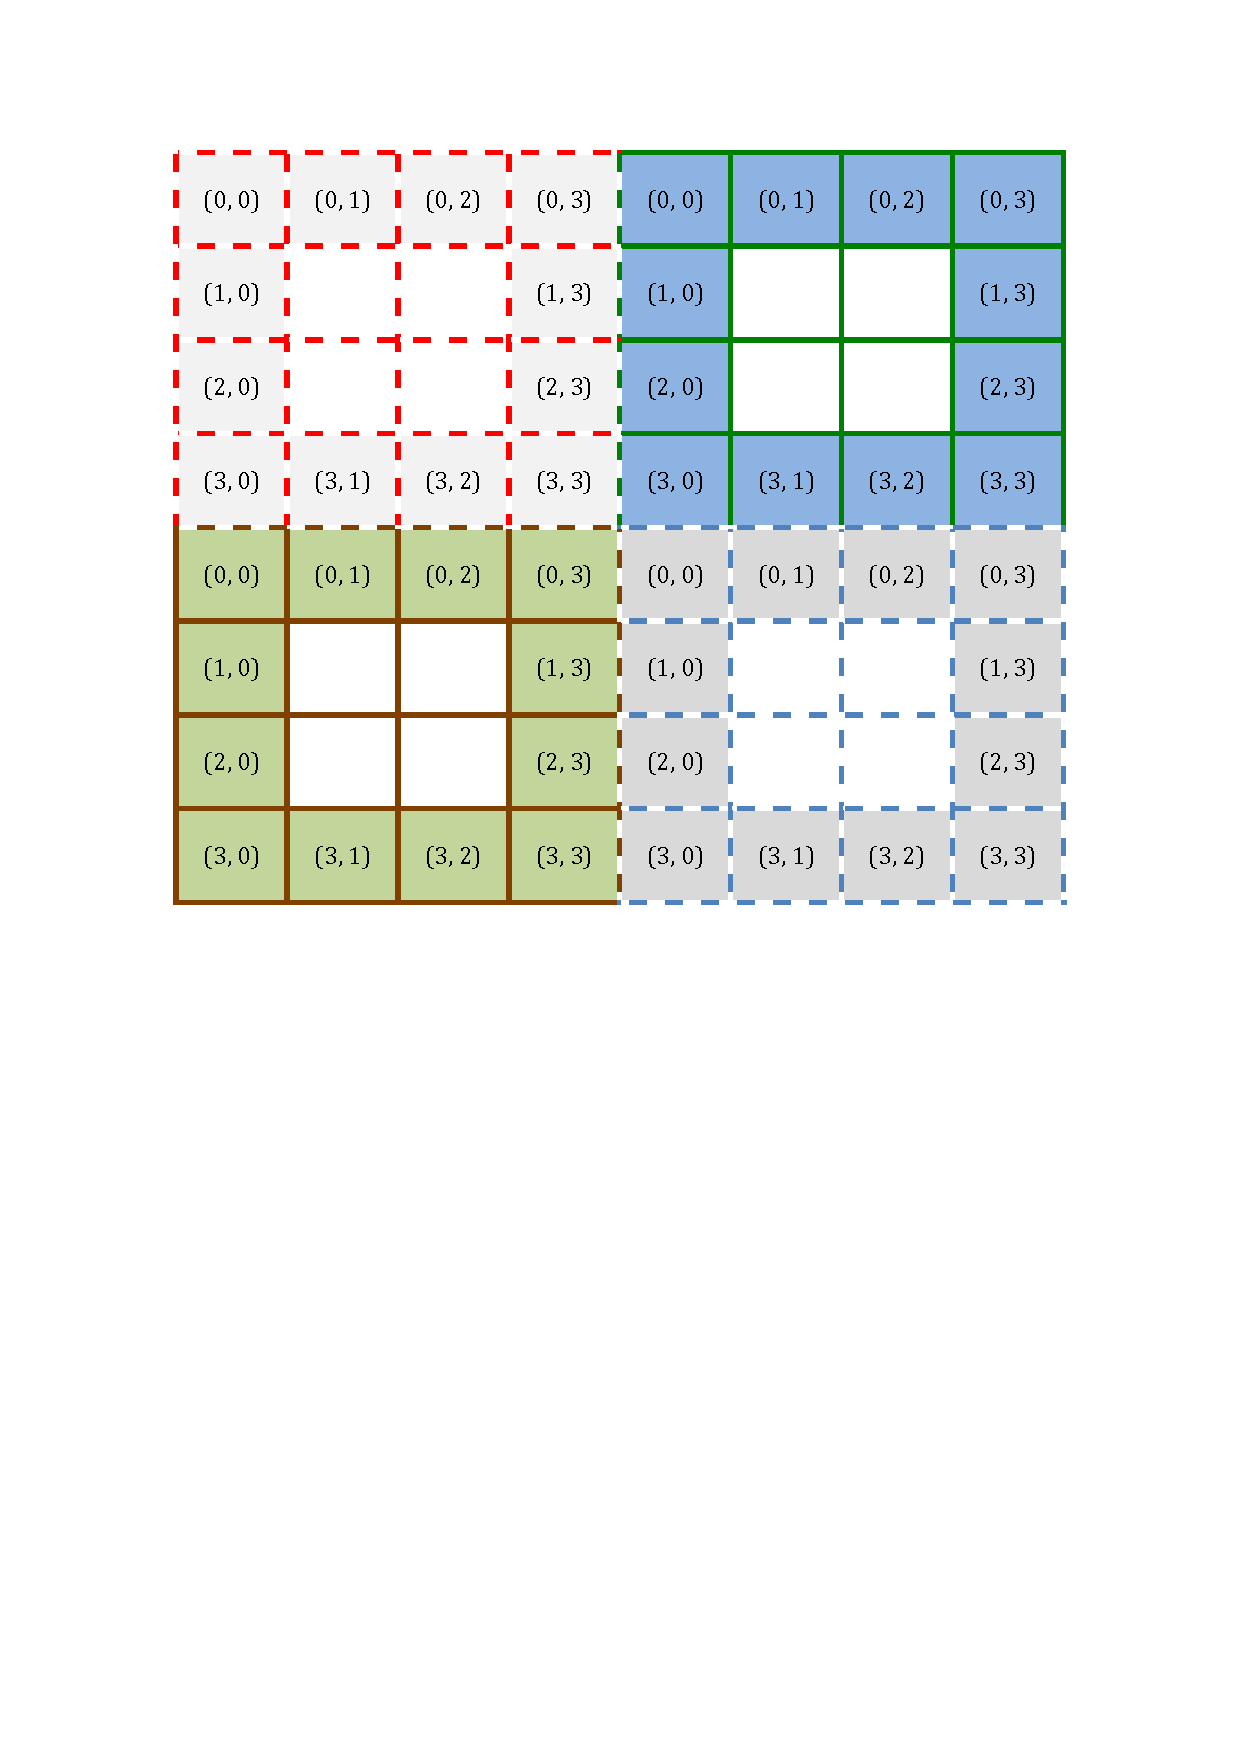
\includegraphics[width=0.475\textwidth]{fig/ht-grid-3.pdf}
   			\hfill
   		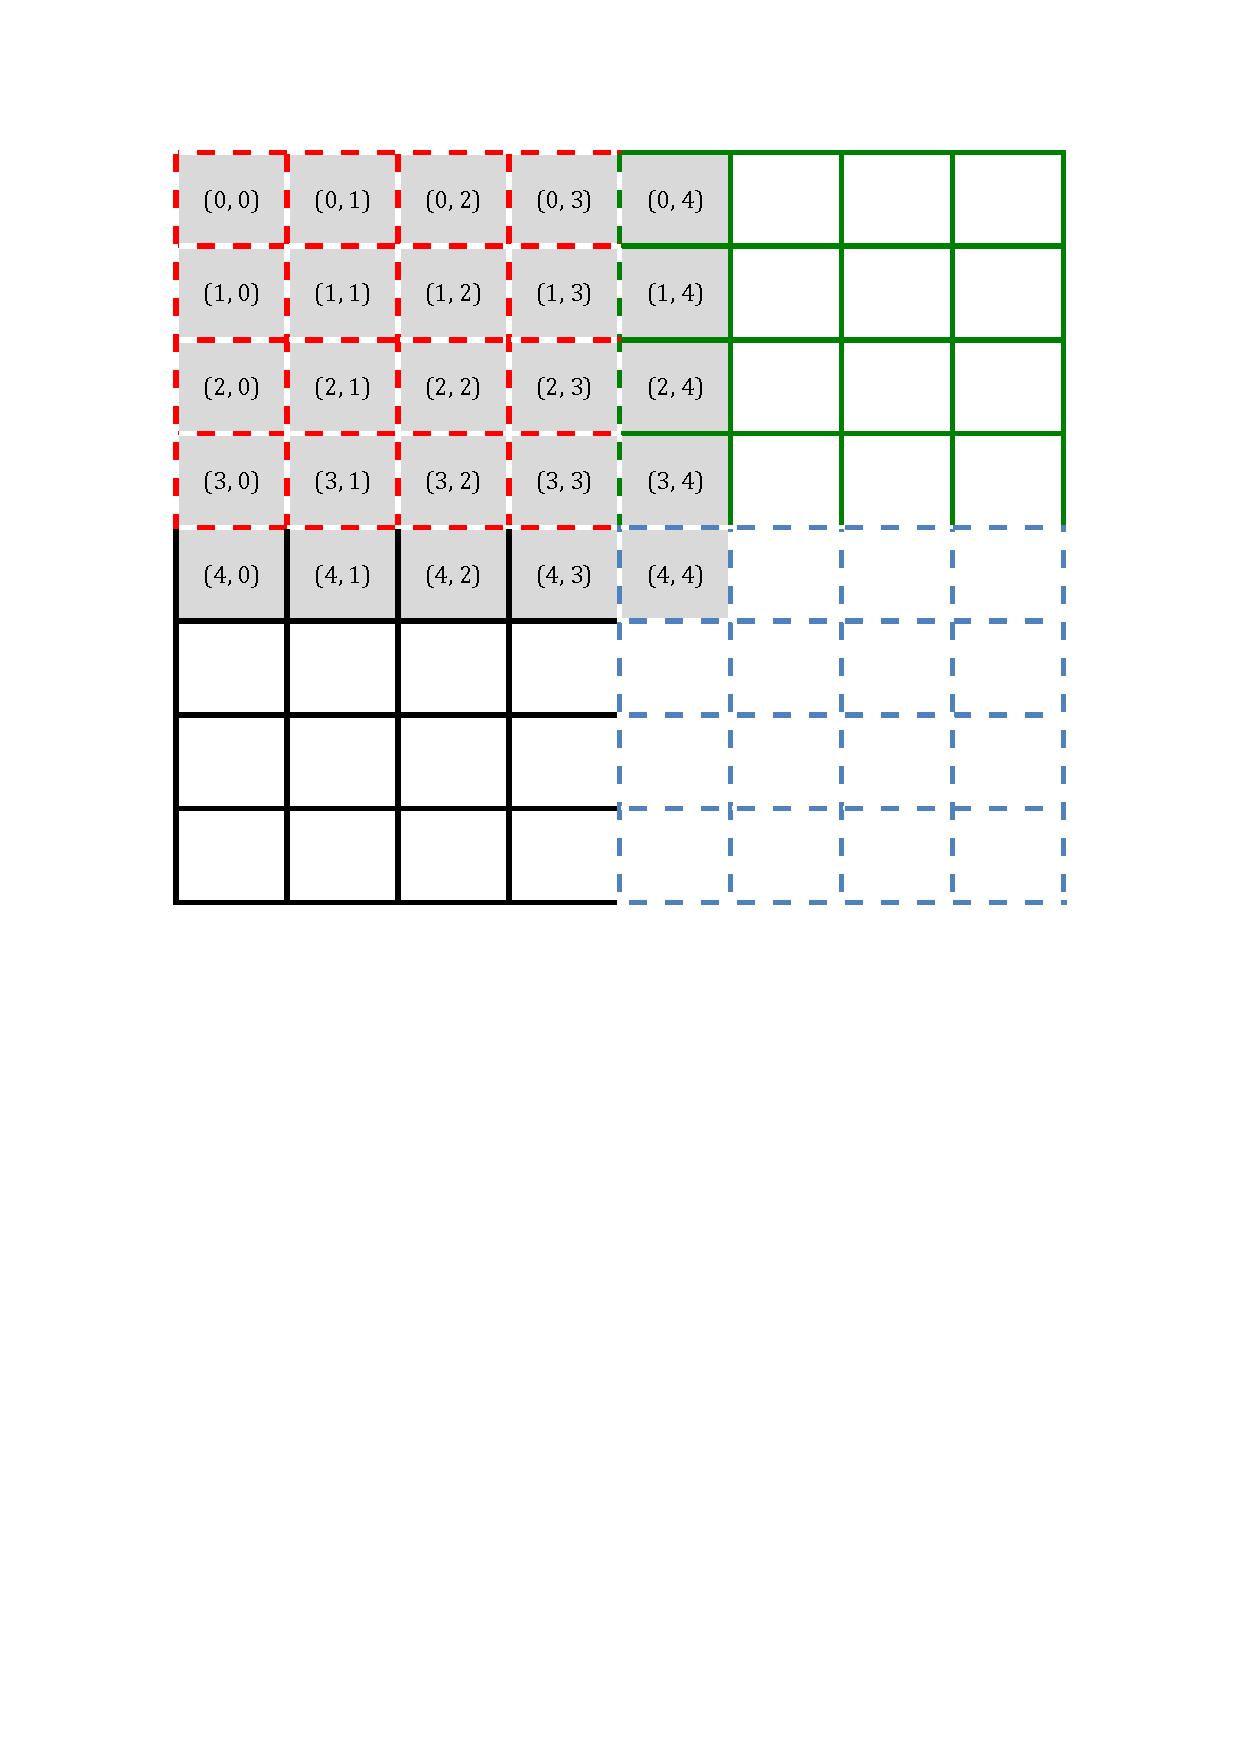
\includegraphics[width=0.475\textwidth]{fig/ht-grid-4.pdf}

      \end{figure} 
      Data visualization after sharing ghost cells among the processors. 		    
  \end{block}
}
%%%%%%%%%%%%%%%%%%%%%%%%%%%%%%%%%%%%%%%%%%%%%%%%%%%%%%%%%%%%%%%%%%%%%%%%%%%%%%%%%%%%%%%%%%

%%%%%%%%%%%%%%%%%%%%%%%%%%%%%%%%%%%%%%%%%%%%%%%%%%%%%%%%%%%%%%%%%%%%%%%%%%%%%%%%%%%%%%%%%%
%%%%%%%%%%%%%%%%%%%%%%%%%%%%%%%%%%%%%%%%%%%%%%%%%%%%%%%%%%%%%%%%%%%%%%%%%%%%%%%%%%%%%%%%%%
\subsubsection{Bioinformatics problems}
%%%%%%%%%%%%%%%%%%%%%%%%%%%%%%%%%%%%%%%%%%%%%%%%%%%%%%%%%%%%%%%%%%%%%%%%%%%%%%%%%%%%%%%%%%
%%%%%%%%%%%%%%%%%%%%%%%%%%%%%%%%%%%%%%%%%%%%%%%%%%%%%%%%%%%%%%%%%%%%%%%%%%%%%%%%%%%%%%%%%%

%%%%%%%%%%%%%%%%%%%%%%%%%%%%%%%%%%%%%%%%%%%%%%%%%%%%%%%%%%%%%%%%%%%%%%%%%%%%%%%%%%%%%%%%%%
\frame[t]
{
  \frametitle{Parallel decomposition}
  	\framesubtitle{Bioinformatics}
		\begin{block}{Biological data can be big}
		A few examples:
		\begin{itemize}
		\item Gene expression data: DNA microarrays now provide tens of thousands of values per sample.
			\begin{figure}[!htb]
      			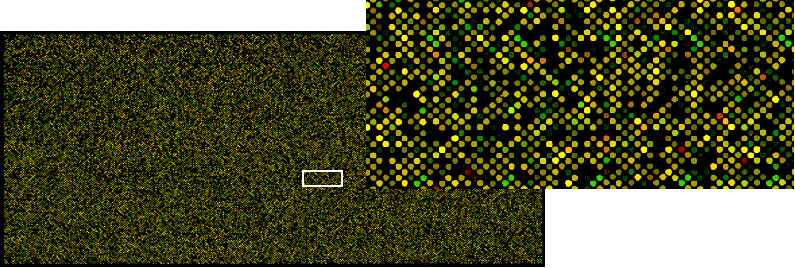
\includegraphics[width=230pt]{fig/cag_48_genome.jpg}	
			\end{figure}  
		\item Protein X-ray Crystallography.
		\item DNA Sequencing.
		\end{itemize}
		\end{block}
}


\frame[t]
{
  \frametitle{Parallel decomposition}
  	\framesubtitle{Bioinformatics}
		\begin{block}{DNA sequencing technology is outpacing Moore's Law}
			\begin{figure}[htb]
      			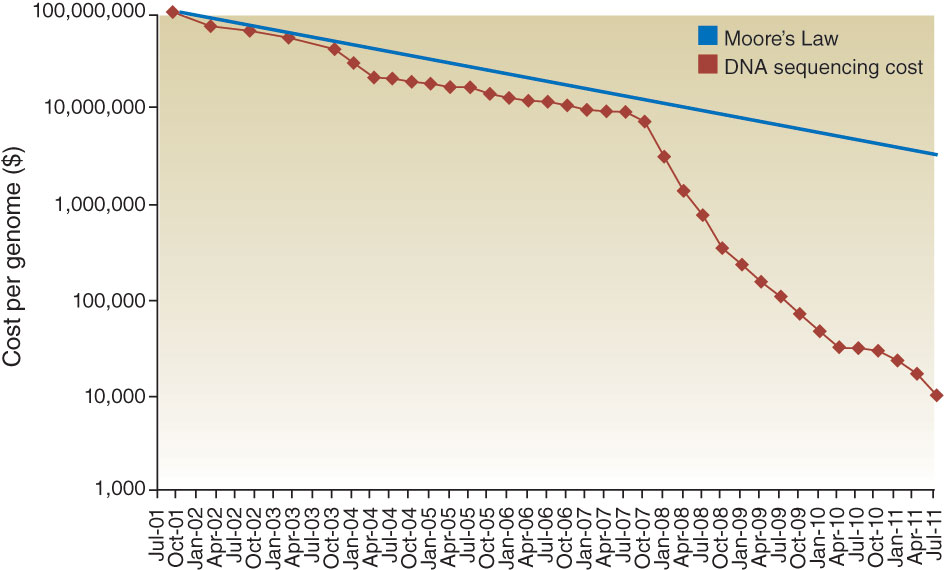
\includegraphics[width=0.9\textwidth]{fig/nbt.jpg}	
			\end{figure}  
		\end{block}
}


\frame[t]
{
  \frametitle{Parallel decomposition}
  	\framesubtitle{Bioinformatics example}
		\begin{block}{Multiple Sequence Alignment}
      Aligning all the related sequences is also computationally intensive even though the 
      amount of data is generally not so large by this step.  
			\begin{figure}[!htb]
      			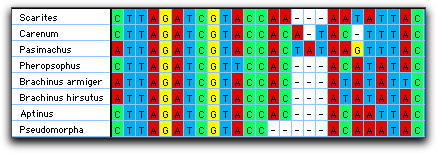
\includegraphics[width=0.9\textwidth]{fig/sequence-alignment.jpg}	
			\end{figure}  
		\end{block}
}

\frame[t]
{
  \frametitle{Parallel decomposition}
  	\framesubtitle{Bioinformatics problem}
		\begin{block}{Pylogenetic Reconstruction}
			Derive a tree of descent from multiple aligned sequences.
			\begin{columns}[t]
			\column{0.45\textwidth}
			\begin{block}{Input}
            \begin{figure}[h]
      			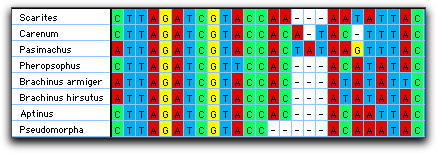
\includegraphics[width=.7\textwidth]{fig/sequence-alignment.jpg}
            \end{figure}
			\end{block}
			\column{0.45\textwidth}
			\begin{block}{Output}
            \begin{figure}[h]
      			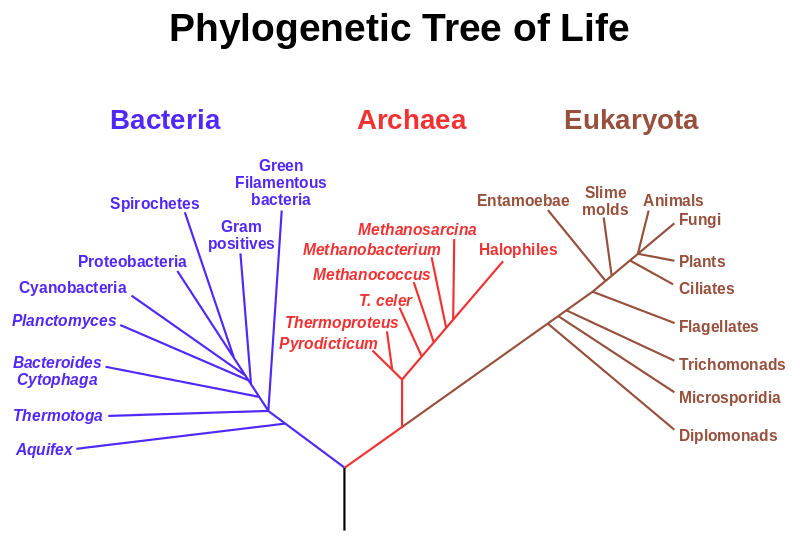
\includegraphics[width=.8\textwidth]{fig/phylogenetic-tree.png}	
            \end{figure}
			\end{block}  
			\end{columns}
		\end{block}
}


\frame[t]
{
\frametitle{Parallel problems - Bioinformatics}
\begin{block}{Evaluating the likelihood of a particular tree}
Given a tree T, alignment A and substitution model S, the core of a likelihood calculation is:
\begin{algorithm}[H]
\begin{algorithmic}
\FOR {each parent node p in T (in a postorder traversal)} \\
%   \IF {p is a leaf}
%      \FOR {each column a and base b} $ L_p_a_b \leftarrow A_p_c = b $ \ENDFOR
%   \ELSE
      \FOR {each alignment column, a} \STATE $ L_p_a \leftarrow [1, 1, 1, 1] $ \ENDFOR
      \FOR {each child node, c, of p} 
         \FOR {each alignment column, a} 
            \STATE $ L_p_a \leftarrow L_p_a \times ( S_p_c \times L_c_a ) $
         \ENDFOR 
      \ENDFOR 
%   \ENDIF
\ENDFOR
\end{algorithmic}
\end{algorithm}
\end{block}
}

\frame[t]
{
  \frametitle{Parallel decomposition}
  	\framesubtitle{Bioinformatics problem}
		\begin{block}{Parallelise tree evaluation by:}
         \begin{itemize}
            \item Tree Branch - to some degree.
            \item Sequence Position - more generally.
         \end{itemize}
      \end{block}
		\begin{block}{Parallelise tree optimisation by:}
         \begin{itemize}
		      \item Parameter Space - e.g., the rate of mutation may take on different values.
            \item Tree Space - the number of possible tree topologies increases quadratically.
         \end{itemize}
		\end{block}
		\note {This slide is intentionally left blank.} 
}

%%%%%%%%%%%%%%%%%%%%%%%%%%%%%%%%%%%%%%%%%%%%%%%%%%%%%%%%%%%%%%%%%%%%%%%%%%%%%%%%%%%%%%%%%%
%%%%%%%%%%%%%%%%%%%%%%%%%%%%%%%%%%%%%%%%%%%%%%%%%%%%%%%%%%%%%%%%%%%%%%%%%%%%%%%%%%%%%%%%%%
\section{Memory classification}
%%%%%%%%%%%%%%%%%%%%%%%%%%%%%%%%%%%%%%%%%%%%%%%%%%%%%%%%%%%%%%%%%%%%%%%%%%%%%%%%%%%%%%%%%%
%%%%%%%%%%%%%%%%%%%%%%%%%%%%%%%%%%%%%%%%%%%%%%%%%%%%%%%%%%%%%%%%%%%%%%%%%%%%%%%%%%%%%%%%%%

%%%%%%%%%%%%%%%%%%%%%%%%%%%%%%%%%%%%%%%%%%%%%%%%%%%%%%%%%%%%%%%%%%%%%%%%%%%%%%%%%%%%%%%%%%
\frame[t]
{
  \frametitle{Parallel programming}
      \begin{block}{Memory Architecture}
      
		Architectural differences between memory architectures have implications 
       	for how we program.   
        \begin{itemize}
            \item Shared-memory systems use a single address space, allowing processors 
            to communicate through variables stored in a shared address space.    
            \item In distributed-memory systems each processor has its own memory 
            module and over a high speed network communications take place.
        \end{itemize}      
   
  \end{block}
}
%%%%%%%%%%%%%%%%%%%%%%%%%%%%%%%%%%%%%%%%%%%%%%%%%%%%%%%%%%%%%%%%%%%%%%%%%%%%%%%%%%%%%%%%%%

%%%%%%%%%%%%%%%%%%%%%%%%%%%%%%%%%%%%%%%%%%%%%%%%%%%%%%%%%%%%%%%%%%%%%%%%%%%%%%%%%%%%%%%%%%
%%%%%%%%%%%%%%%%%%%%%%%%%%%%%%%%%%%%%%%%%%%%%%%%%%%%%%%%%%%%%%%%%%%%%%%%%%%%%%%%%%%%%%%%%%
\subsection{Shared memory}
%%%%%%%%%%%%%%%%%%%%%%%%%%%%%%%%%%%%%%%%%%%%%%%%%%%%%%%%%%%%%%%%%%%%%%%%%%%%%%%%%%%%%%%%%%
%%%%%%%%%%%%%%%%%%%%%%%%%%%%%%%%%%%%%%%%%%%%%%%%%%%%%%%%%%%%%%%%%%%%%%%%%%%%%%%%%%%%%%%%%%

%%%%%%%%%%%%%%%%%%%%%%%%%%%%%%%%%%%%%%%%%%%%%%%%%%%%%%%%%%%%%%%%%%%%%%%%%%%%%%%%%%%%%%%%%%
\frame[t]
{
  \frametitle{Parallel programming}
      \begin{block}{Shared memory}

   \begin{itemize}%[<+-| alert@+>]
	\item Symmetric multiprocessing (SMP) : two or more identical processors share the same memory.
	\item This shared memory may be simultaneously accessed by multiple threads of same program.
	\item The most popular shared memory parallel programming paradigm is OpenMP.
   \end{itemize}
        \begin{center}
 			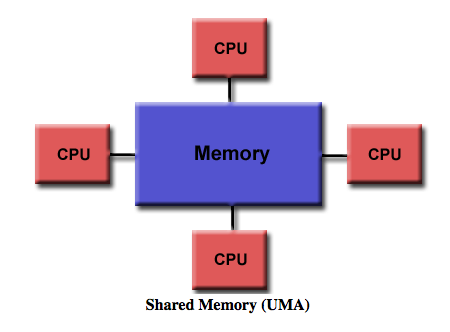
\includegraphics[width=100pt]{fig/shared-memory.png}
   		\end{center}  
   
  \end{block}
}
%%%%%%%%%%%%%%%%%%%%%%%%%%%%%%%%%%%%%%%%%%%%%%%%%%%%%%%%%%%%%%%%%%%%%%%%%%%%%%%%%%%%%%%%%%


%%%%%%%%%%%%%%%%%%%%%%%%%%%%%%%%%%%%%%%%%%%%%%%%%%%%%%%%%%%%%%%%%%%%%%%%%%%%%%%%%%%%%%%%%%
\frame[t]
{
  \frametitle{Parallel programming}
    \framesubtitle{Shared memory}
      \begin{block}{Shared memory: address system}
      
        \begin{center}
 			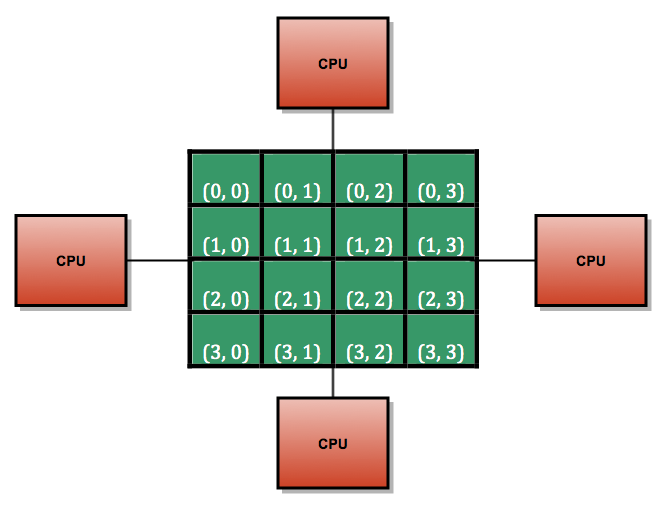
\includegraphics[width=200pt]{fig/shared-archi.png}
   		\end{center}  
   
  \end{block}
}
%%%%%%%%%%%%%%%%%%%%%%%%%%%%%%%%%%%%%%%%%%%%%%%%%%%%%%%%%%%%%%%%%%%%%%%%%%%%%%%%%%%%%%%%%%

%%%%%%%%%%%%%%%%%%%%%%%%%%%%%%%%%%%%%%%%%%%%%%%%%%%%%%%%%%%%%%%%%%%%%%%%%%%%%%%%%%%%%%%%%%
%%%%%%%%%%%%%%%%%%%%%%%%%%%%%%%%%%%%%%%%%%%%%%%%%%%%%%%%%%%%%%%%%%%%%%%%%%%%%%%%%%%%%%%%%%
\subsection{Distributed memory}
%%%%%%%%%%%%%%%%%%%%%%%%%%%%%%%%%%%%%%%%%%%%%%%%%%%%%%%%%%%%%%%%%%%%%%%%%%%%%%%%%%%%%%%%%%
%%%%%%%%%%%%%%%%%%%%%%%%%%%%%%%%%%%%%%%%%%%%%%%%%%%%%%%%%%%%%%%%%%%%%%%%%%%%%%%%%%%%%%%%%%

%%%%%%%%%%%%%%%%%%%%%%%%%%%%%%%%%%%%%%%%%%%%%%%%%%%%%%%%%%%%%%%%%%%%%%%%%%%%%%%%%%%%%%%%%%
\frame[t]
{
  \frametitle{Parallel programming}
      \begin{block}{Distributed memory}

   \begin{itemize}%[<+-| alert@+>]
	\item Multiple-processor computer system in which each process has its own private memory. 
	\item Computational tasks can only operate on local data.
	\item If remote data is required, the computational task must communicate with one or more remote processors.
	\item The most popular distributed memory programming paradigm is MPI.
   \end{itemize}
        \begin{center}
 			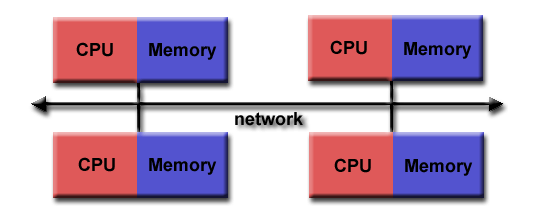
\includegraphics[width=150pt]{fig/dist-memory.png}
   		\end{center}     
  \end{block}
}
%%%%%%%%%%%%%%%%%%%%%%%%%%%%%%%%%%%%%%%%%%%%%%%%%%%%%%%%%%%%%%%%%%%%%%%%%%%%%%%%%%%%%%%%%%


%%%%%%%%%%%%%%%%%%%%%%%%%%%%%%%%%%%%%%%%%%%%%%%%%%%%%%%%%%%%%%%%%%%%%%%%%%%%%%%%%%%%%%%%%%
\frame[t]
{
  \frametitle{Parallel programming}
      \begin{block}{Distributed memory: address system}
        \begin{center}
 			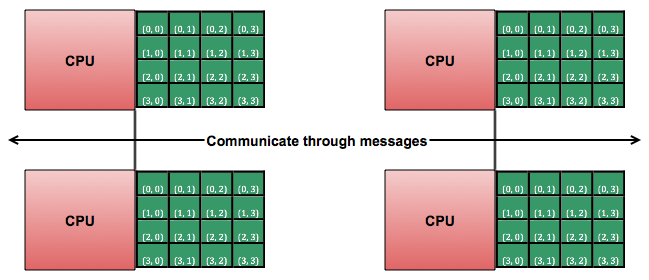
\includegraphics[width=300pt]{fig/distri-archi.png}
   		\end{center}     
  \end{block}
}
%%%%%%%%%%%%%%%%%%%%%%%%%%%%%%%%%%%%%%%%%%%%%%%%%%%%%%%%%%%%%%%%%%%%%%%%%%%%%%%%%%%%%%%%%%


%%%%%%%%%%%%%%%%%%%%%%%%%%%%%%%%%%%%%%%%%%%%%%%%%%%%%%%%%%%%%%%%%%%%%%%%%%%%%%%%%%%%%%%%%%
\frame[t]
{
  \frametitle{Parallel programming}
      \begin{block}{OpenMP vs MPI}
        \begin{itemize}
            \item   OpenMP 
                \begin{itemize}
            		\item  Easy to parallelise existing codes without much coding effort.
        			\item Look for iterative operations.
        			\item Use OpenMP directives (#pragma) to parallelise it. 
        			These create threads that will run in parallel 
        			on different cores of the same node.
        		\end{itemize}
      
      		\item MPI
      		      \begin{itemize}
      		      	\item If you want to scale your application beyond the maximum 
      		      	number of cores available on a node. 
      
      				\item MPI is only a standard for message passing libraries based 
      				on the consensus of the MPI Forum. 
      				\item There are different implementations of it. 
      				\item Popular implementations include: OpenMPI, MPICH, Intel MPI.       
           		\end{itemize}
        \end{itemize}
  \end{block}
}
%%%%%%%%%%%%%%%%%%%%%%%%%%%%%%%%%%%%%%%%%%%%%%%%%%%%%%%%%%%%%%%%%%%%%%%%%%%%%%%%%%%%%%%%%%


%%%%%%%%%%%%%%%%%%%%%%%%%%%%%%%%%%%%%%%%%%%%%%%%%%%%%%%%%%%%%%%%%%%%%%%%%%%%%%%%%%%%%%%%%%
\frame[t]
{
  \frametitle{Parallel programming}
\begin{block}{Hybrid programming model}
    \begin{itemize}
      	\item Mix and match OpenMP and MPI:
    	\begin{itemize}   	 
      		\item OpenMP manages the workload on each (SMP) node.
      		\item MPI facilitates communication among multiple nodes over the network.
      	 \end{itemize} 
      	 
      	 \item The best of both worlds:
    	 \begin{itemize}   	 
      	 	\item OpenMP ensures efficient utilization of shared memory within a (SMP) node. 
      	 	\item MPI facilitates efficient inter-node operations and sending of complex
      	 	data structures.
    	 \end{itemize}        	 	 
      	 
    \end{itemize} 
  \end{block}
}
%%%%%%%%%%%%%%%%%%%%%%%%%%%%%%%%%%%%%%%%%%%%%%%%%%%%%%%%%%%%%%%%%%%%%%%%%%%%%%%%%%%%%%%%%%

%%%%%%%%%%%%%%%%%%%%%%%%%%%%%%%%%%%%%%%%%%%%%%%%%%%%%%%%%%%%%%%%%%%%%%%%%%%%%%%%%%%%%%%%%%
\frame[t]
{
  \frametitle{Parallel programming}
    \begin{block}{}
        \begin{center}
            \Huge Thank You \\
      		Questions?
		\end{center}
	\end{block}
}
%%%%%%%%%%%%%%%%%%%%%%%%%%%%%%%%%%%%%%%%%%%%%%%%%%%%%%%%%%%%%%%%%%%%%%%%%%%%%%%%%%%%%%%%%%



%%%%%%%%%%%%%%%%%%%%%%%%%%%%%%%%%%%%%%%%%%%%%%%%%%%%%%%%%%%%%%%%%%%%%%%%%%%%%%%%%%%%%%%%%%
\frame[t]
{
  \frametitle{Acknowledgments}
        \begin{itemize}
            \item Slides developed by:
              \begin{itemize}
              	\item Jaison Paul Mulerikkal, PhD
              	\item Peter Maxwell
				\end{itemize}
        \end{itemize}
  
\begin{center}
\vspace*{0.5cm}
 
\includegraphics[width=210pt]{NeSI_img/nesi_logo.jpg}\\
 
\includegraphics[width=50pt]{NeSI_img/logo-u-of-a.jpg}
 
\includegraphics[width=50pt]{NeSI_img/logo-u-of-c.jpg}
 
\includegraphics[width=50pt]{NeSI_img/logo-niwa.jpg}
 
\includegraphics[width=50pt]{NeSI_img/logo-ministry-of-si.jpg} 
 
\includegraphics[width=50pt]{NeSI_img/logo-manaaki-whenua.jpg}
 
\includegraphics[width=50pt]{NeSI_img/logo-u-of-o.jpg}
\end{center}
}
%%%%%%%%%%%%%%%%%%%%%%%%%%%%%%%%%%%%%%%%%%%%%%%%%%%%%%%%%%%%%%%%%%%%%%%%%%%%%%%%%%%%%%%%%%
%%%%%%%%%%%%%%%%%%%%%%%%%%%%%%%%%%%%%%%%%%%%%%%%%%%%%%%%%%%%%%%%%%%%%%%%%%%%%%%%%%%%%%%%%%

%%%%%%%%%%%%%%%%%%%%%%%%%%%%%%%%%%%%%%%%%%%%%%%%%%%%%%%%%%%%%%%%%%%%%%%%%%%%%%%%%%%%%%%%%%
\frame[t]
{
  \frametitle{Acknowledgments}
      \begin{block}{Reference}
 		\begin{itemize}
   		 	\item  \href{https://computing.llnl.gov/tutorials/parallel_comp/}
   		 	{Blaise Barney, Introduction to Parallel Computing, LLNL.}
   		 	\item Dr John Rugis, NeSI.    
 		\end{itemize}
   
  \end{block}
}
%%%%%%%%%%%%%%%%%%%%%%%%%%%%%%%%%%%%%%%%%%%%%%%%%%%%%%%%%%%%%%%%%%%%%%%%%%%%%%%%%%%%%%%%%%


\end{document} 
